\documentclass[12pt,oneside]{paper}

\usepackage{listings}
\renewcommand{\lstlistingname}{saucecode}

\lstset{%
  language={C},
  basicstyle={\small},%
  identifierstyle={\small},%
  commentstyle={\small\itshape},%
  keywordstyle={\small\bfseries},%
  ndkeywordstyle={\small},%
  stringstyle={\small\ttfamily},
  frame={tb},
  breaklines=true,
  columns=[l]{fullflexible},%
  numbers=left,%
  xrightmargin=0zw,%
  xleftmargin=3zw,%
  numberstyle={\scriptsize},%
  stepnumber=1,
  numbersep=1zw,%
  lineskip=-0.5ex%
}



% タイトル
\title{長距離飛行するストロー飛行機の製作}
\author{北川鼓太朗}

\begin{document}
% 行間
\setlength{\baselineskip}{9truemm}

%文字間
\kanjiskip=.53zw plus 3pt minus 3pt
\xkanjiskip=.53zw plus 3pt minus 3pt

% 目次
\tableofcontents
%\newpage
% 本文
\chapter{はじめに}

\section{研究の背景}
当研究室では飛行ロボットコンテストに出場するために飛行機の設計・製作を行っている.今年度は一般部門に出場するために固定翼の作成と、マルチコプター部門に出場するためにマルチコプターの製作を行った.固定翼の部品はアクリルを用いておりレーザ加工を行い制作されている.(図\ref{fig:acril})レーザ加工を用いる事によって部品加工時間が短縮され、また部品の大量生産を可能にした.また同じようにマルチコプターの胴体の部分をレーザ加工で加工してあるためこちらも大量生産・製作時間の短縮を実現している.(図\ref{fig:doutai}).以上の製作方法を用いて機体を制作した後、プログラムなど制御関係を終わらし大会参加を行い決勝でよい成績を残す事が目的となっている.大会には出場出来たものの決勝には進出することが出来ず予選敗退だった。敗退の要因であった縦安定についてストロー飛行機製作を通して学ぼうと考えた.
\begin{figure}[htbp]
  \begin{center}
    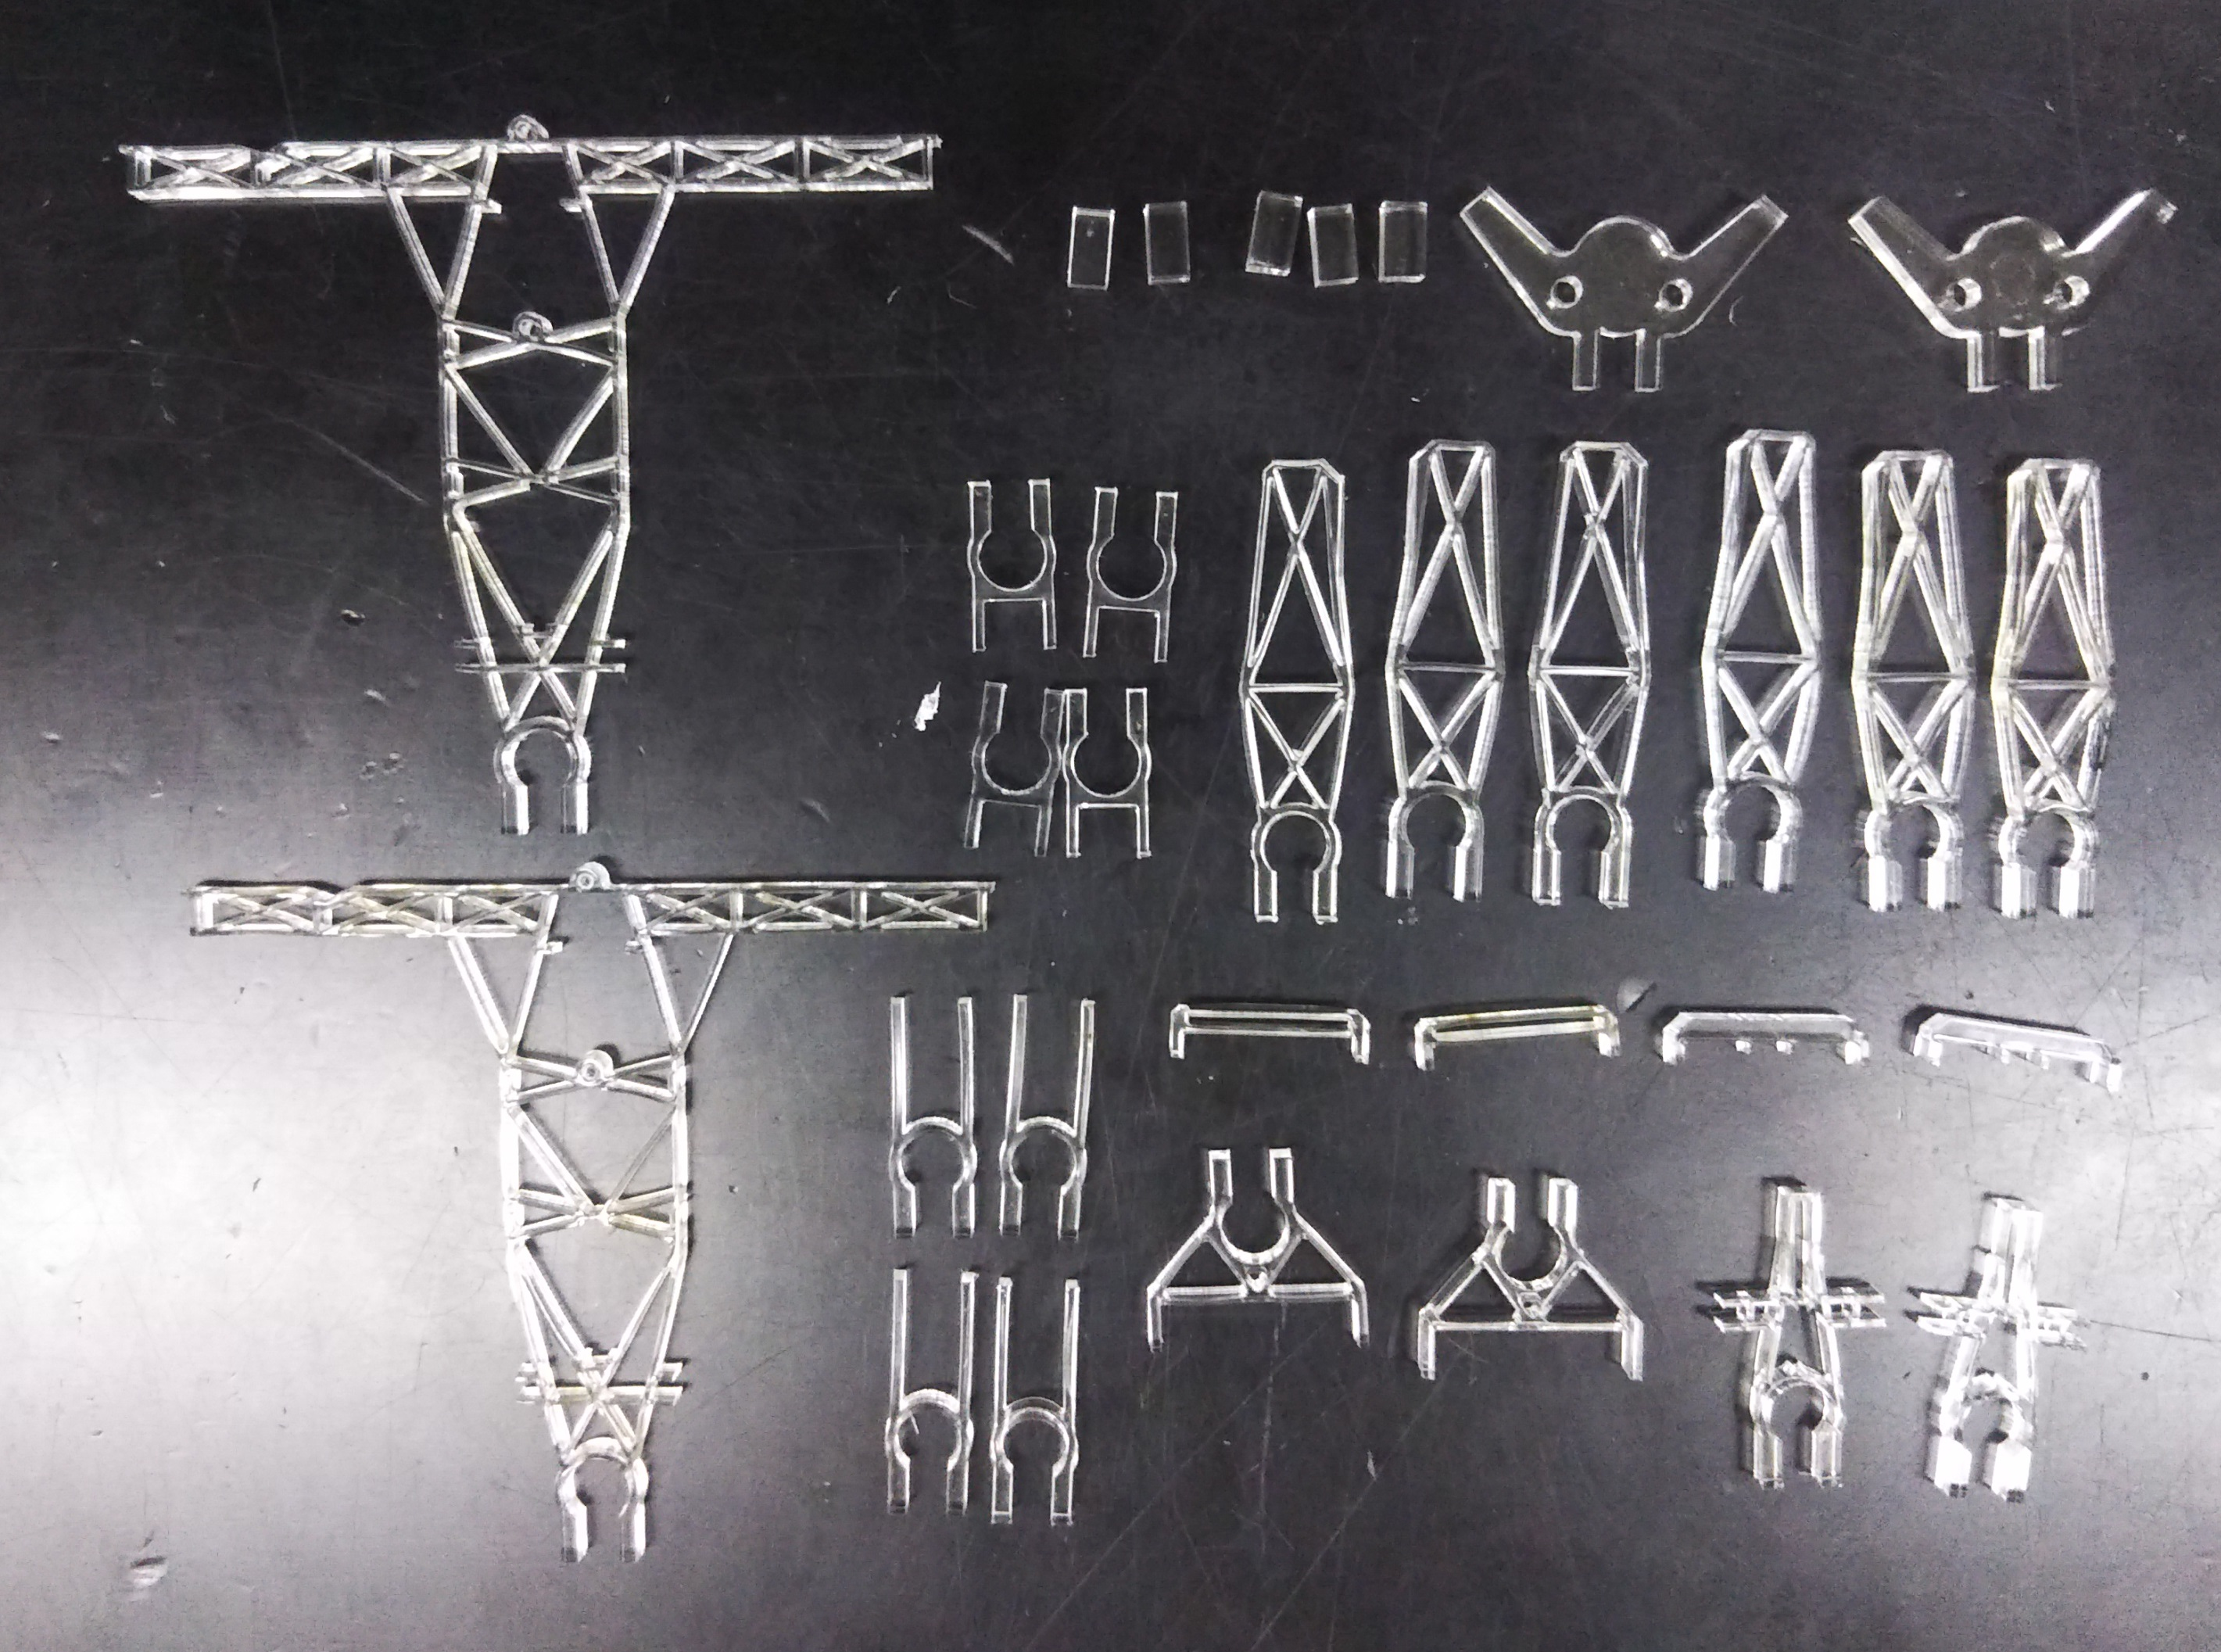
\includegraphics[width=80mm]{acril.jpg}
    \end{center}
  \caption{アクリル部品}
 \label{fig:acril}
\end{figure}

\begin{figure}[htbp]
  \begin{center}
    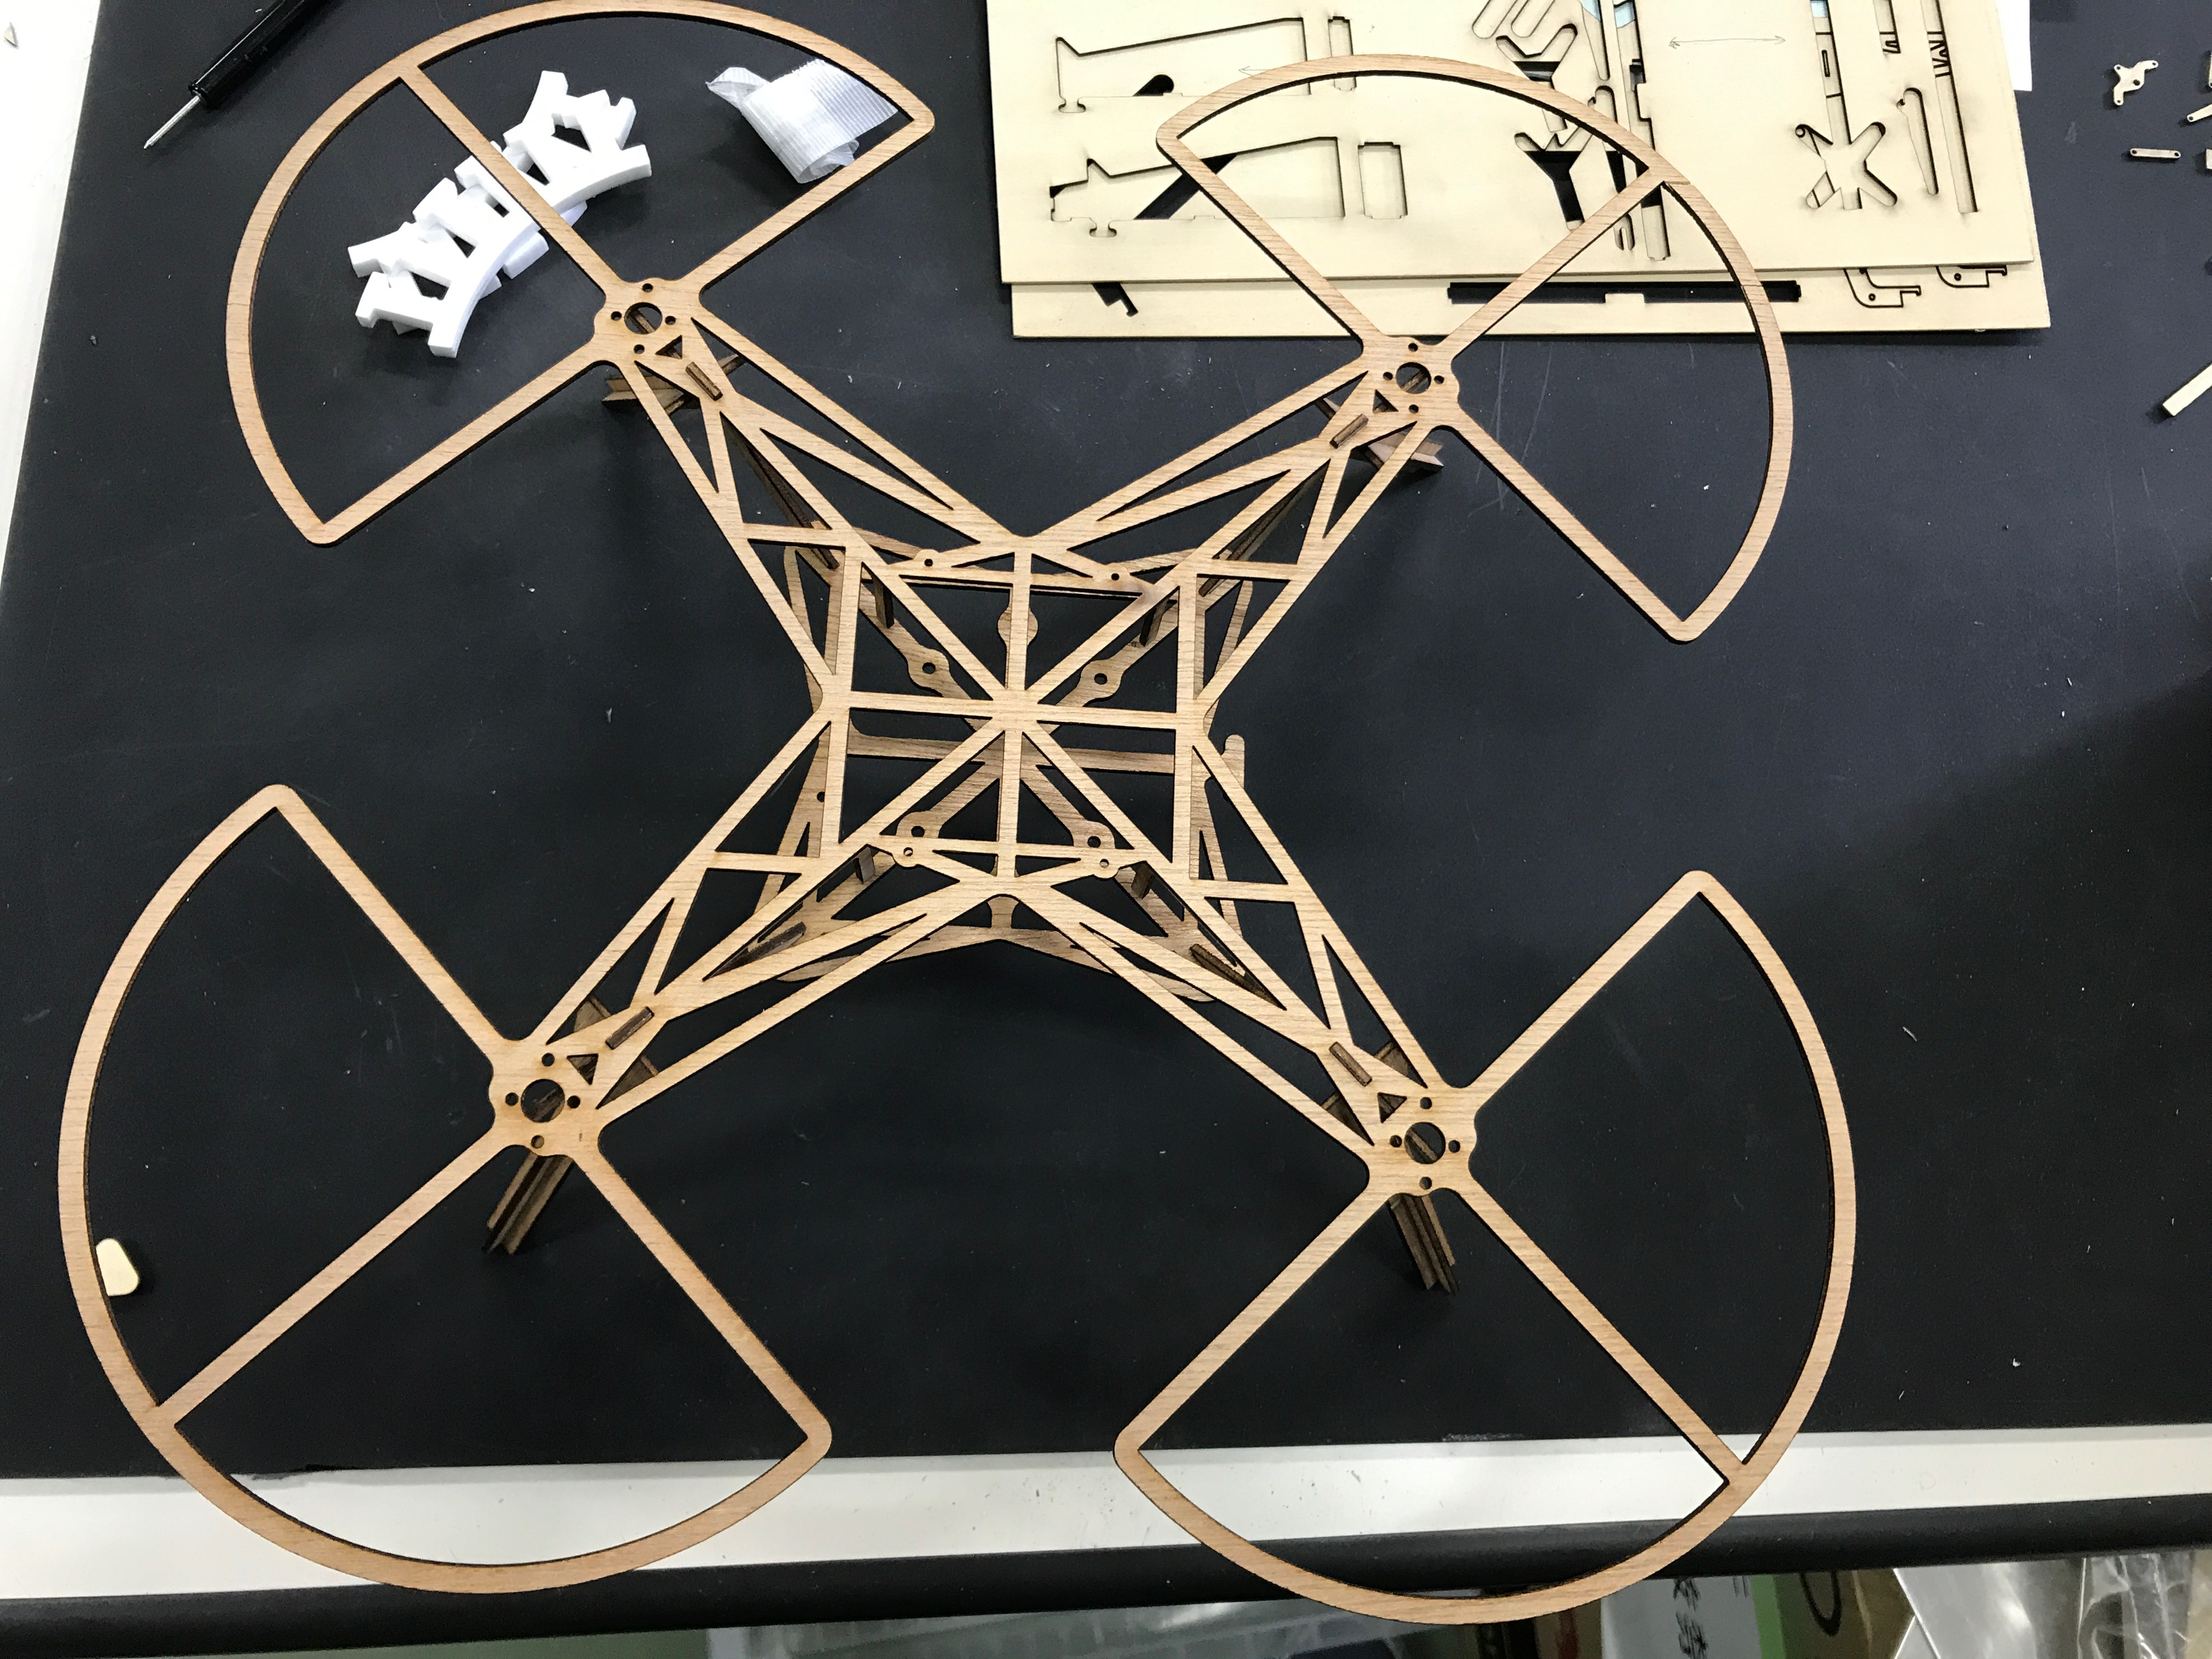
\includegraphics[width=80mm]{doutai.jpg}
    \end{center}
  \caption{胴体}
 \label{fig:doutai}
\end{figure}

\section{研究の目的}
大会出場時は飛行機の構成や原理など分かっていなかったため大会後、飛行機を設計するために知っておかないといけない構成や原理を理解するために簡単な飛行機を作り飛行機が飛行出来る原理の勉強を行いたいと考えていた.
しかし身近に原理を理解できる教材がなかったため,安く手に入りやすい材料を使い飛行原理を知らない人でも分かる教材の開発を作る事を目的としている.



\section{本論文の構成}
1章では,本研究の背景と簡略化した概要を示す.2章では飛行理論について,胴体の決定方法と絡めながら説明する.3章ではストロー飛行機の製作方法について述べる.4章では製作したストロー飛行機の飛行試験の結果について述べる.5章では本研究の結論を示す.


\chapter{実験用飛行機の試作機の設計}
初めて飛行機を作るにあたり,胴体の選定方法や飛行性能を実験を用いて調べた.この章では胴体について述べる.

\section{一般的な飛行機の形状}
一般的な飛行機は主翼・尾翼・垂直尾翼の三翼から成っている.多くの飛行機はテーパ翼という翼幅に沿って翼弦長が直線的に変化するもの通常は翼端側が翼弦長が小さくなるため、「先細翼」とも呼ばれている形を用いる事が多い.他にも楕円の形をした楕円翼,長方形の形をした矩形翼などがある.今回は胴体を一般的な円柱状の形と似ている長さ180mm,直径5mmのストローを胴体とし、翼の形をテーパ翼ときめて翼を作りその後貼り合わせる事でストロー飛行機を製作した.

\section{ストローの良否の選定}
ストロー飛行機作りはとても繊細な作業であるため胴体として使うストローにも注意が必要である.そのため今回は良いストローを見分けるための方法を紹介していきたいと思う.
方法としてはまずストローを平らな平面に置き転がす.このとき真っすぐなストローだと綺麗に転がるが曲がっているストローの場合,綺麗に転がらずカタカタと音がする.以上の方法により真っすぐなストローを見分ける.下記に注意点を述べる.
\begin{itemize}
\item 真っすぐなストロー以外使用しない

\item 判断が出来ない場合は他の人にも確認してもらう

\item 真っすぐなストローと真っがっているストローの区別を出来るようにする

\item 少しでも真っがっている場合でも使用しない

\end{itemize}

\section{モデルに選んだ機体の説明}
普段よく飛行機と呼んでいるが飛行機には様々な種類が存在する.表に主な飛行機の種類と大まかな用途を説明する\ref{tab:airplane}.

\begin{table}[H]
 \begin{center}
   \caption{飛行機の種類}
   \begin{tabular}[htbp]{|c|c|}
    \hline
    種類&用途 \\
    \hline
    旅客機&旅行など長距離の移動に使用\\
    \hline
    戦闘機&戦闘に特化した飛行機で戦争の時などに使用\\
    \hline
    垂直離着陸機&滑走路を必要としないため比較的狭い場所でもよい\\
    \hline
    爆撃機&戦争の時などに多くの爆弾類などを搭載させた飛行機\\
    \hline
    貨物機&主に貨物輸送を行う飛行機のこと\\
    \hline
    偵察機&相手を偵察するときに使用\\
    \hline
    
    \end{tabular}
   \label{tab:airplane}
  \end{center}
\end{table}

上記のように飛行機にも様々な種類があり機体によって滑空性能が変化する.そこで今回モデルに選んだ機体は研究目的である長い距離飛ぶ飛行機を達成できると思われる戦闘機を選定した.選定理由としては戦闘機は主に戦争の時使用されるため運動性能が他の飛行機より優れていると考えられる.また世界各国で生産されているためそれぞれの機体に正確な差があると思ったため差が分かりやすい戦闘機を選定した.
今回は日本の戦闘機である零戦とアメリカ海軍の戦闘機であるグラマンを選定した.次の章で2機の特徴を記す.

\subsection{零戦}
零戦とは零式艦上戦闘機の略称であり、第二次世界大戦の時日本海軍の戦闘機として活躍していた.太平洋戦争初期の頃は世界最高水準の戦闘機で航続距離が長く、軽快で運動性能に富んでいた戦闘機である.また世界最大の航続距離で当時の世界一流戦闘機の2~3倍、落下タンクを付ければ5倍もあった。軽い機体で普通の戦闘機より1000kg以上軽い。零戦の図を図\ref{fig:reisen}に示す.

\begin{figure}[htbp]
  \begin{center}
    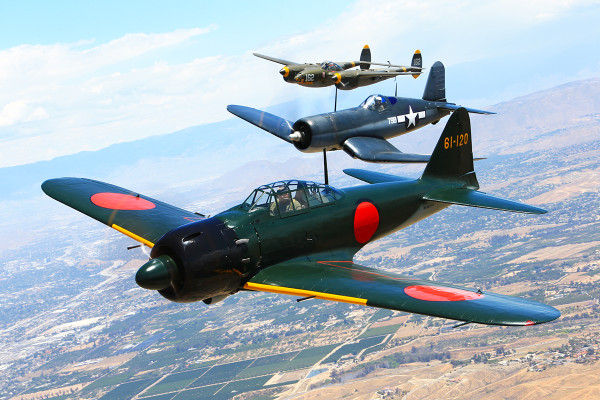
\includegraphics[width=140mm]{reisen.JPG}
    \end{center}
  \caption{零戦実機}
 \label{fig:reisen}
\end{figure}

\subsection{F6F ヘルキャット}
ヘルキャットとはアメリカの航空機会社であるグラマン社が製造した第二次大戦中アメリカ海軍の主力戦闘機である.良好な運動性能、急降下性能を有していたため日本の航空戦力を撃破するのに最も貢献した機体である.ズーム上昇は頑丈さゆえに急降下で速度を稼げるヘルキャットの方が零戦よりも優れている.さらに、急降下性能、武装、防弾性能、横転性能、旋回性能も、時速400km以下の速度域以外では零戦より優れていた.
ヘルキャットの図を図\ref{fig:F6F}に示す.

\begin{figure}[htbp]
  \begin{center}
    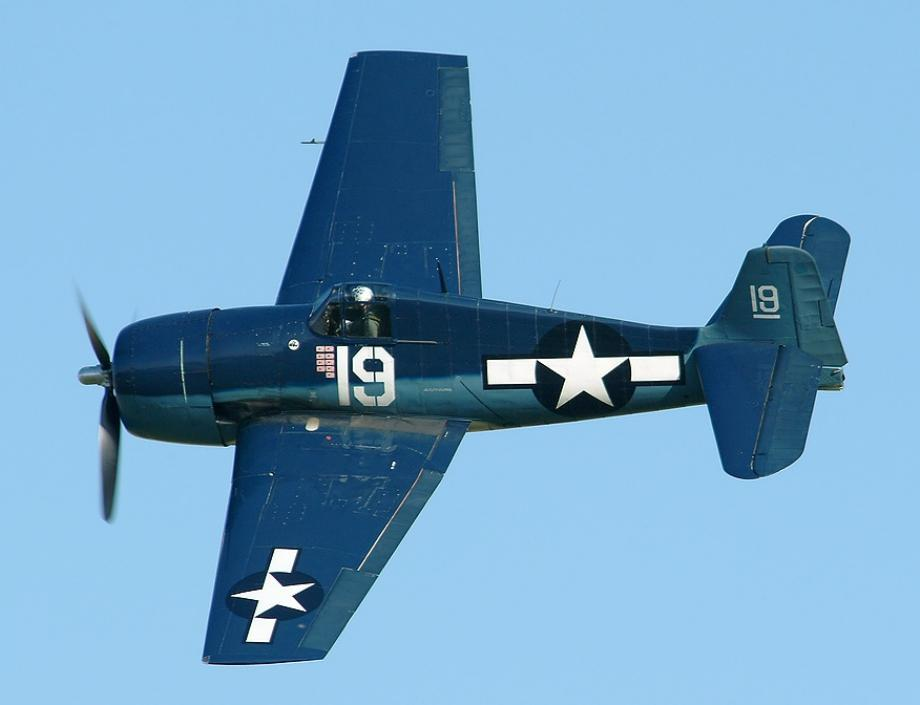
\includegraphics[width=140mm]{F6F.JPG}
    \end{center}
  \caption{ヘルキャット実機}
 \label{fig:F6F}
\end{figure}

\section{試作機の図面の製作方法}
図面を制作する際,まずインターネットで零戦とヘルキャットの図面を検索し図面を印刷する.その後図面の寸法を定規を用いて測り,(ストローの全長/図面の全長)*測りたい部分の長さの公式を用いて長さを算出した後CADを用いて図面を作成する.
算出の結果,零戦の主翼の全長は205.8mm,尾翼の全長は88.8mm,垂直尾翼の全高は30.4mmという結果になった.寸法入りの図面を図\ref{fig:mainwing},\ref{fig:tail}に示す.また零戦完成モデルの写真を図\ref{fig:sen}に示す.

\begin{figure}[htbp]
  \begin{center}
    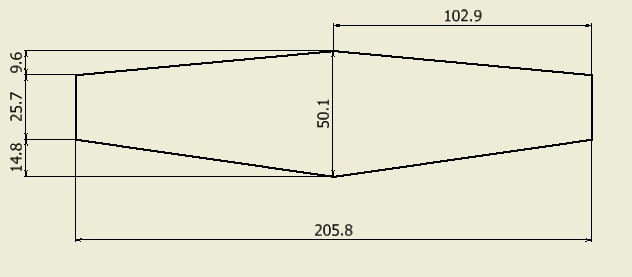
\includegraphics[width=140mm]{mainwing.JPG}
    \end{center}
  \caption{零戦主翼図面}
 \label{fig:mainwing}
\end{figure}

\begin{figure}[htbp]
  \begin{center}
    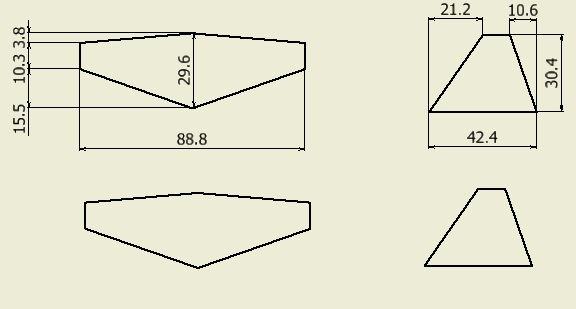
\includegraphics[width=140mm]{tail.JPG}
    \end{center}
  \caption{零戦図面}
 \label{fig:tail}
\end{figure}

\begin{figure}[htbp]
  \begin{center}
    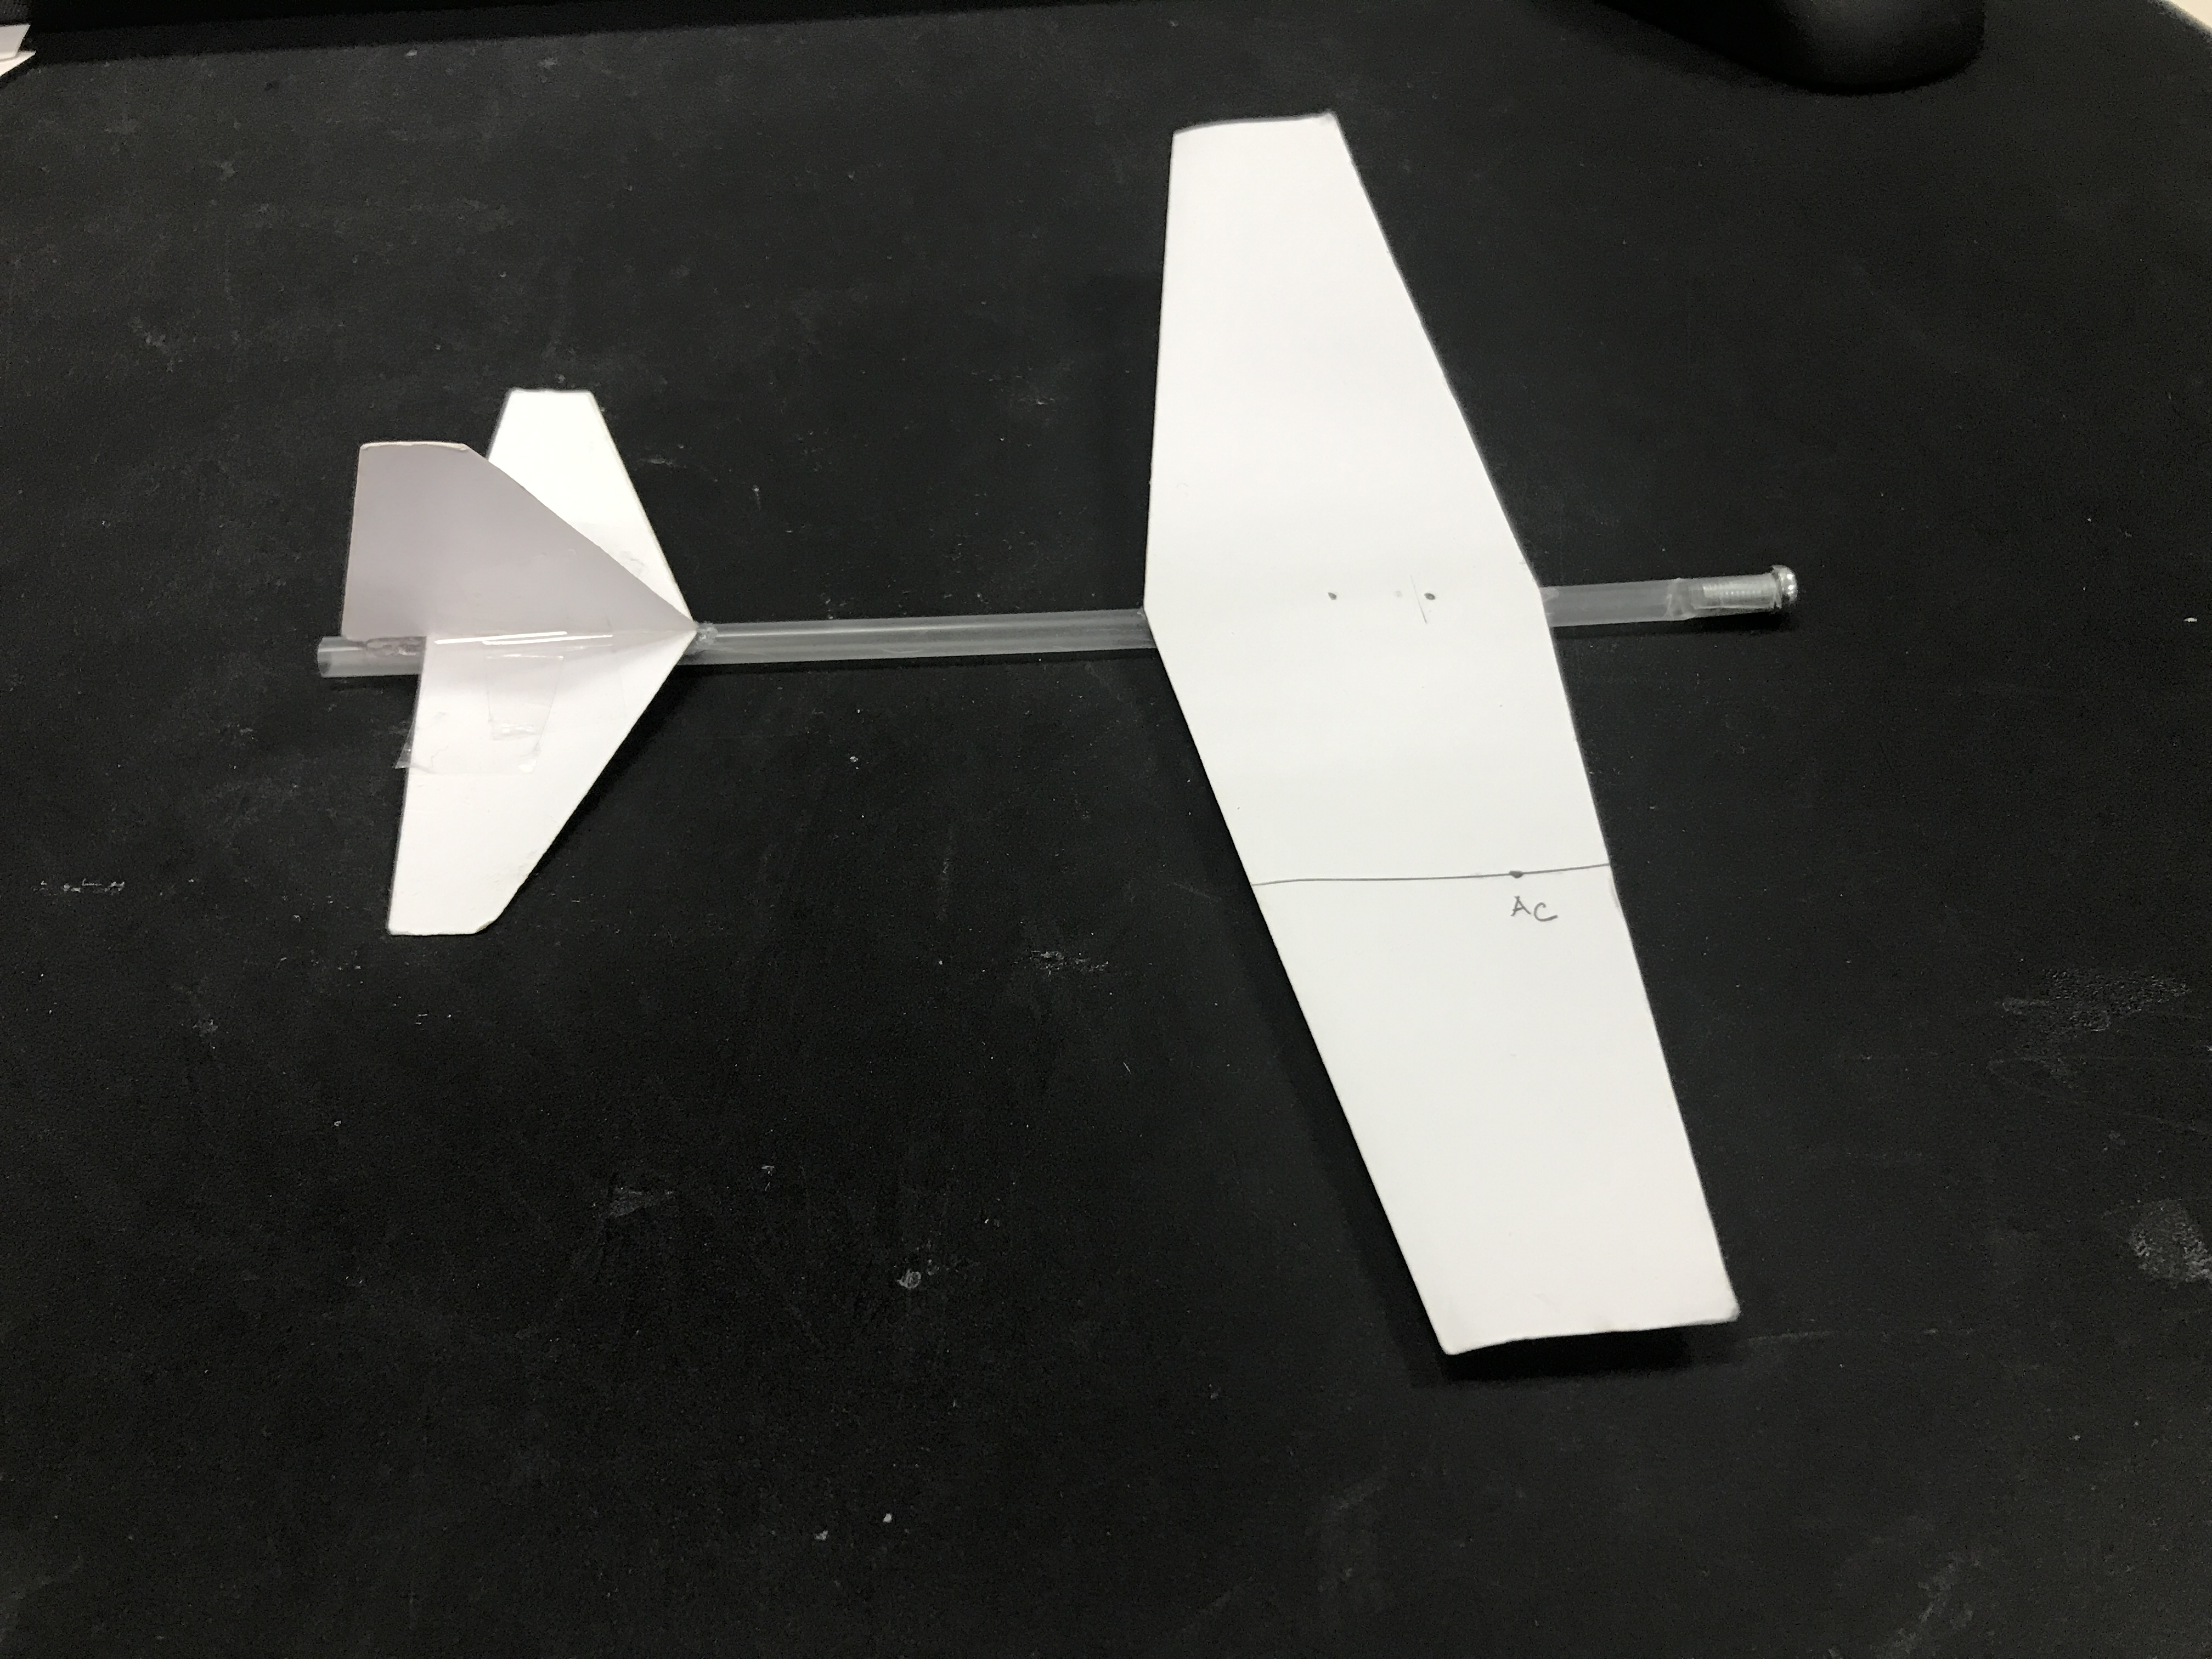
\includegraphics[width=140mm]{sen.JPG}
    \end{center}
  \caption{零戦}
 \label{fig:sen}
\end{figure}


次にヘルキャットの算出を行った結果,主翼の全長は242.4mm,尾翼の全長は108.2mm,垂直尾翼の全高は28.5mmという結果になった.寸法入り図面を図\ref{fig:guramanmainwing},\ref{fig:guramantail}に示す.またヘルキャット完成モデルの写真を図\ref{fig:man}に示す.

\begin{figure}[htbp]
  \begin{center}
    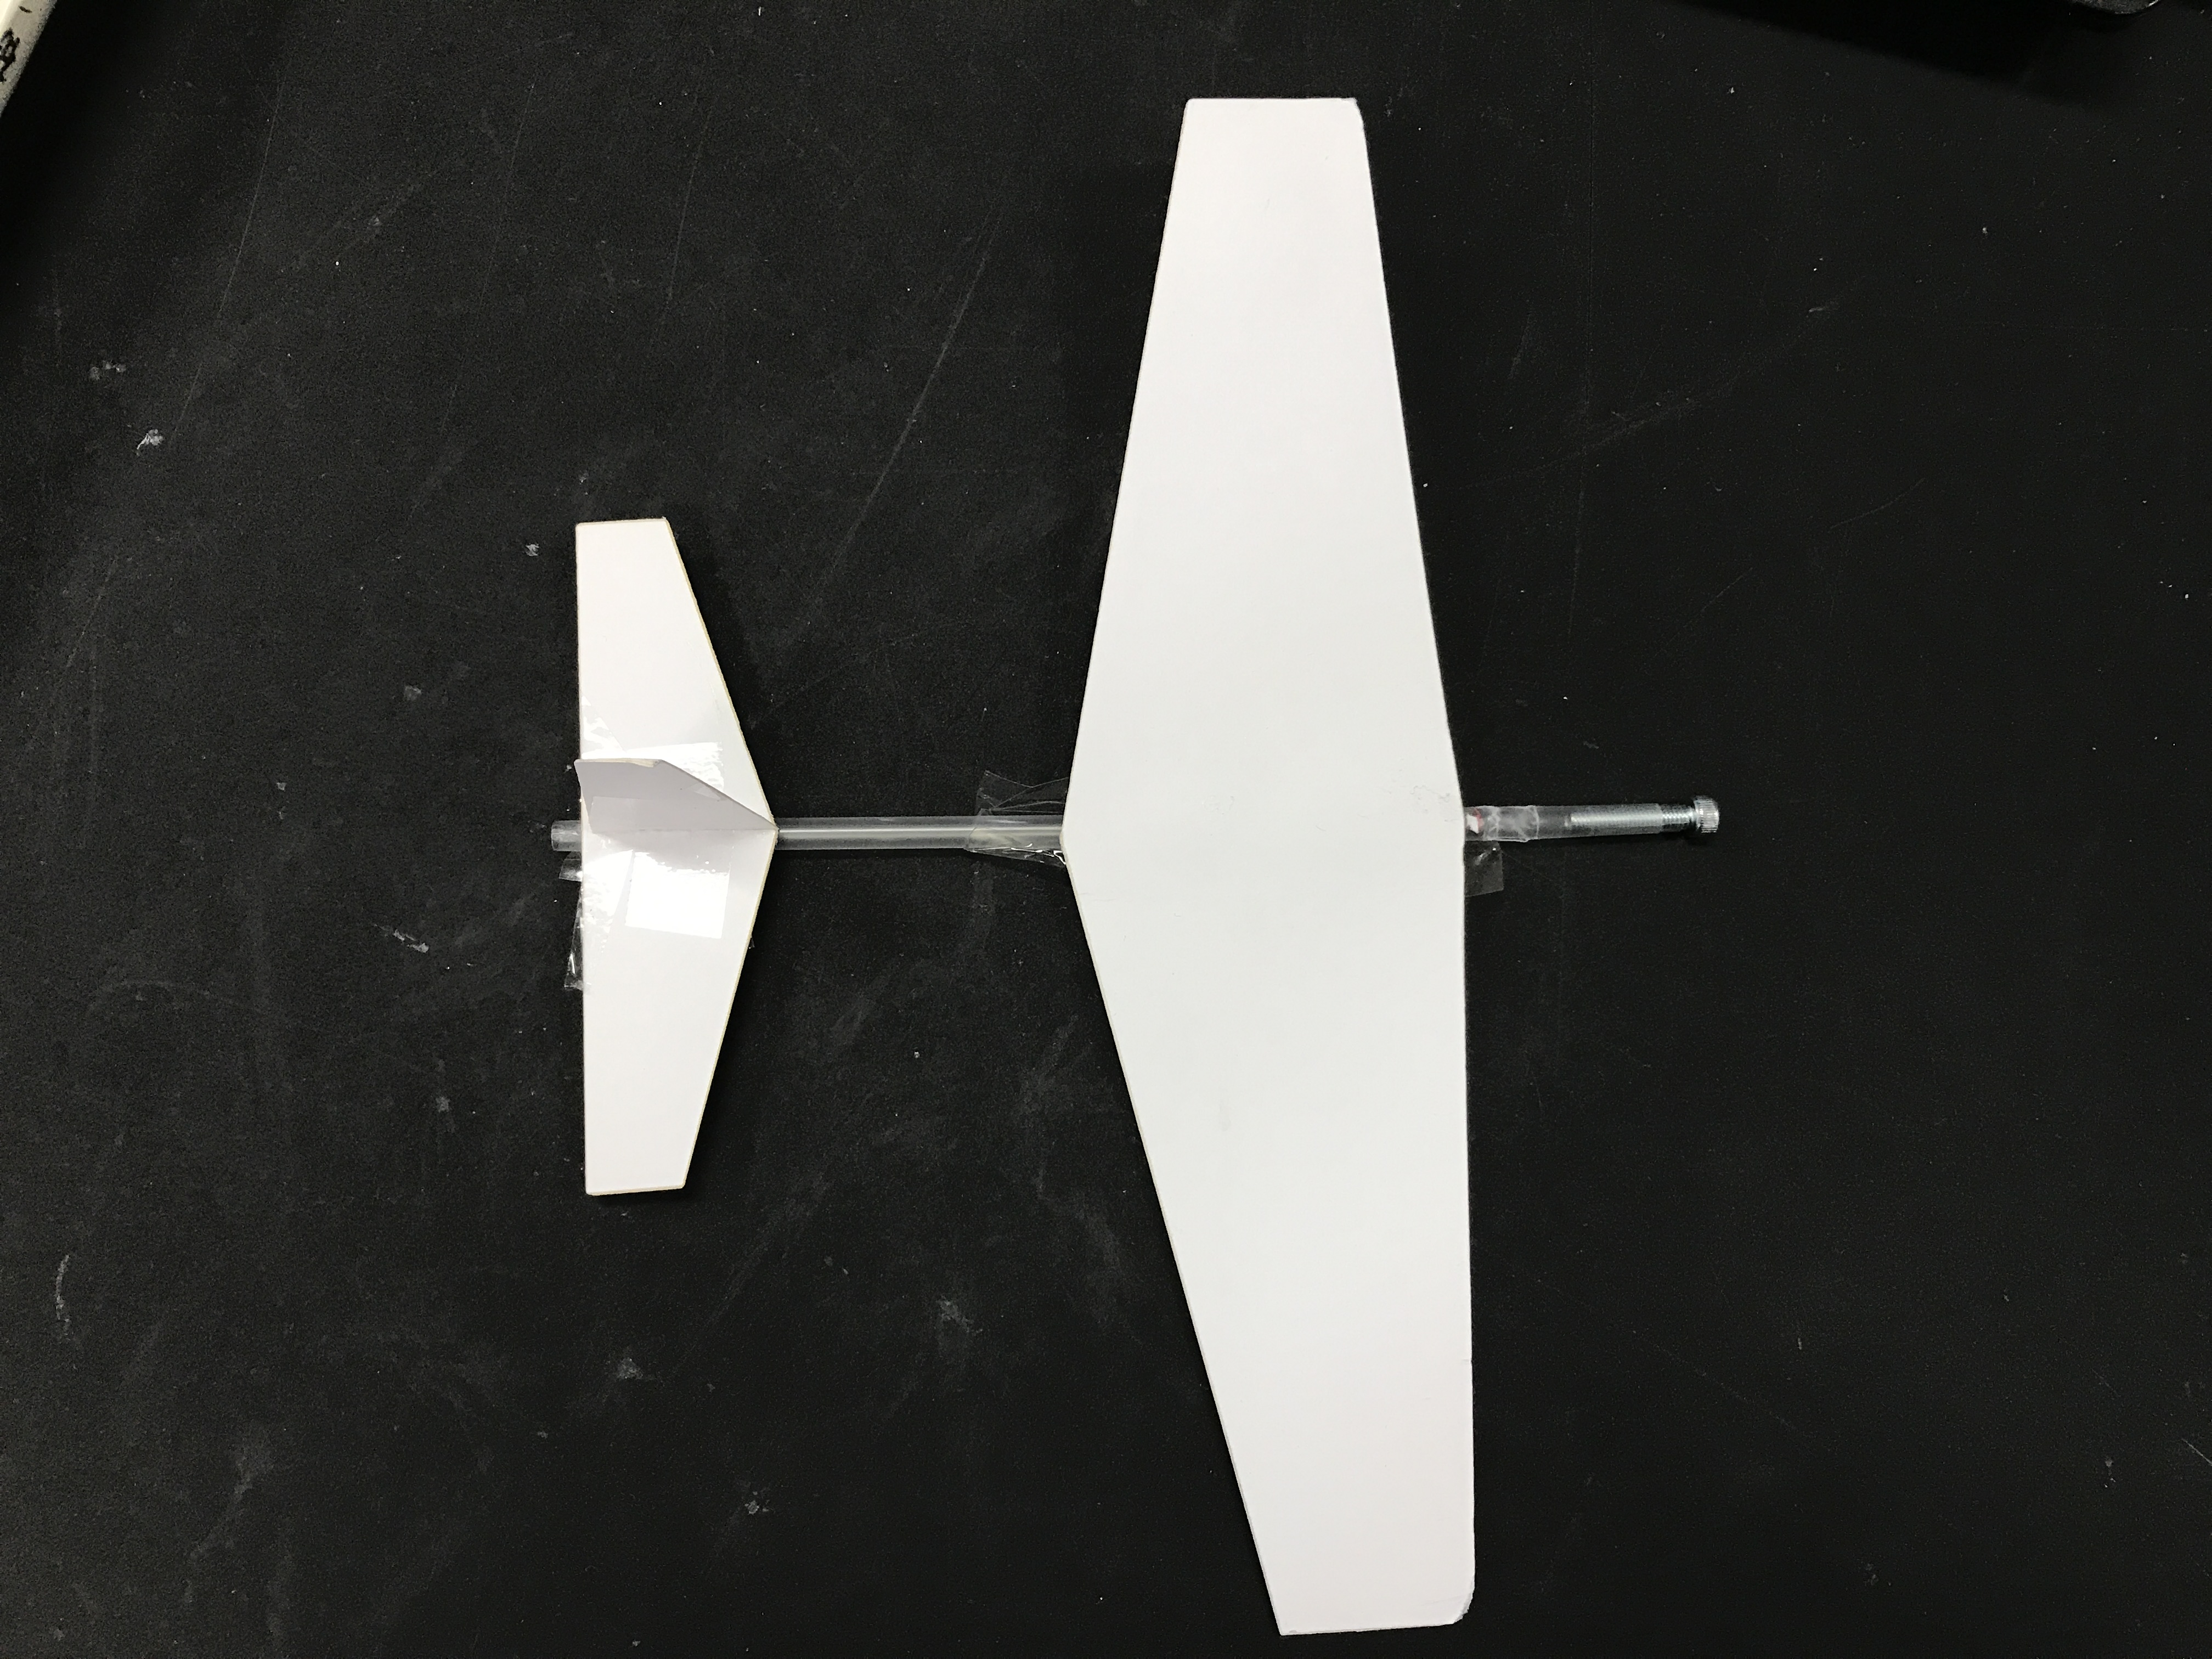
\includegraphics[width=140mm]{man.JPG}
    \end{center}
  \caption{ヘルキャット}
 \label{fig:man}
\end{figure}

\begin{figure}[htbp]
  \begin{center}
    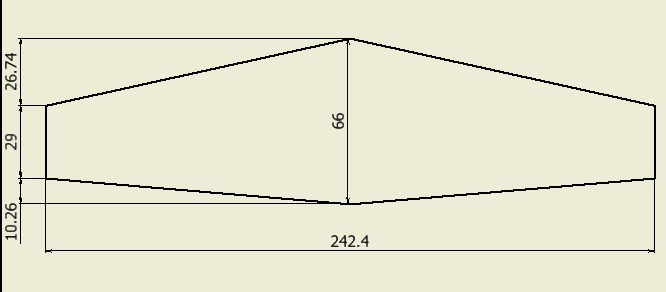
\includegraphics[width=140mm]{guramanmainwing.JPG}
    \end{center}
  \caption{ヘルキャット主翼図面}
 \label{fig:guramanmainwing}
\end{figure}

\begin{figure}[htbp]
  \begin{center}
    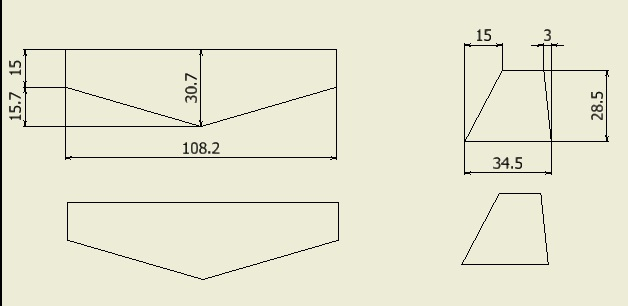
\includegraphics[width=140mm]{guramantail.JPG}
    \end{center}
  \caption{ヘルキャット図面}
 \label{fig:guramantail}
\end{figure}

図面から零戦よりもヘルキャットの方が翼が大きいことが分かる.またテーパ比は零戦が0.513,ヘルキャットが0.439,翼面積は零戦が7800,ヘルキャットが11514という結果になった.このことからテーパ比は零戦の方が大きいが翼面積はヘルキャットの方が大きいことが分かる.以上より零戦は機体の軽快性に優れていると考えヘルキャットは機体の安定性に優れていると考える.

\section{飛行機の縦の安定性}
飛行機が安定して真っすぐ飛ぶためには機体の重心位置がとても関係がある.もし重心位置を考えなかった場合,機体が宙返りしたり飛んだ瞬間頭から落ちる現象が発生する.したがって作図と計算を用いて重心位置の算出を行った.
\subsection{空力中心}
主翼はある一定の中心点を中心に揚力が発生するとみなすことが出来る.その点を空力中心と呼ぶ.空力中心を求めるためには計算でも求める事が可能だがテーパ翼では作図を用いて求める事が多い.したがって今回は作図を用いて求める方法を紹介したいと思う.
まず初めに主翼の片翼だけの図面を印刷する.その後下図\ref{fig:yoku}のように作図を行う.交点から約25割の位置が空力中心である.交点から垂直に線を伸ばし翼中央と交わった所がその翼の一番揚力が発生する位置である.
したがって今回作成した零戦の場合,空力中心位置が後ろから130mm,重心位置が後ろから121mmの位置にあるため機体が頭上げの動作を行う構造となっている.頭上げを行うと機体が宙返りしたりするため真っすぐ機体が飛ぶ確率が低い.そのため空力中心と重心位置を出来るだけ近づけた方が安定して機体が飛ぶ事が出来る.
\begin{figure}[htbp]
  \begin{center}
    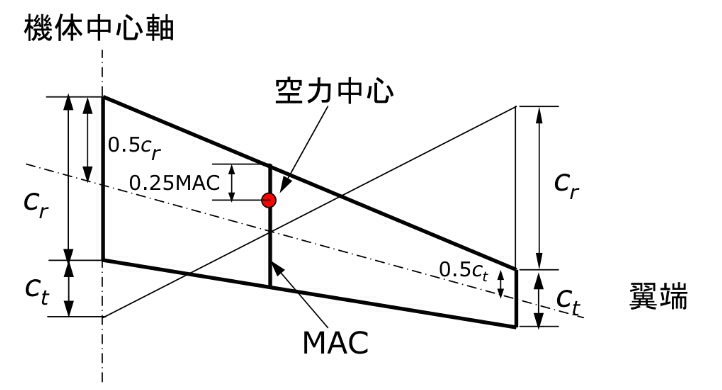
\includegraphics[width=140mm]{yoku.JPG}
    \end{center}
  \caption{空力中心の求め方}
 \label{fig:yoku}
\end{figure}


\chapter{ストロー飛行機の作成}



\section{翼の加工方法}
\subsection{カッター}
前章で製作した図面を印刷しカッターで切り出す.最初は定規を当てず切っていたが微妙なズレが生じ,飛行距離に差が生じた.そのため定規を当てながら切る事でズレを生じさせないようにした.しかしカッターを用いる欠点としては一機作るために約30~40分かかるため多大な時間がかかる・大量生産が出来ない・ズレが生じるという欠点があったため違う加工方法を模索することにした.次に同じカッターでも図面の線を極限まで細くし,カッターを定規に当てながら加工を行った.結果は以前より格段に加工精度が上昇したが手作業のため直角が出し切れず,ズレが生じてしまった.そのため次にレーザ加工を実践することに決めた.

\subsection{レーザ加工}
次にレーザ加工を用いて加工する事にした.まずCAD上で作成した翼を図面化し,その後dxfファイルに変換することでレーザ加工ファイルを作る.まず加工する前に実験を行い最適な数値の決定を行った.実験の結果を表\ref{tab:experiment}に示す.

\begin{table}[H]
 \begin{center}
   \caption{レーザ実験結果}
   \begin{tabular}[htbp]{|c|c|c|}
    \hline
    スピード(S)&パワー(W)&結果 \\
    \hline
    5.0&20&切れるが少し焦げ臭い\\
    \hline
    6.0&20&焦げないが約1割が切り取りにくい\\
    \hline
    7.0&20&約5割が切れない\\
    \hline
    8.0&20&約7割が切れない\\
    \hline
    5.0&19&焦げ臭さが薄くなった\\
    \hline
    6.0&19&約1.5割が切れない\\
    \hline
    7.0&19&約6割が切れない\\
    \hline
    8.0&19&約8割が切れない\\
    \hline
    5.0&18&加工後ススが出る\\
    \hline
    6.0&18&約2割が切れない\\
    \hline
    7.0&18&約7割が切れない\\
    \hline
    8.0&18&約9割が切れない\\
    \hline
    5.0&17&綺麗な加工断面が得られるが多少ススが出る\\
    \hline
    6.0&17&約3割が切れない\\
    \hline
    7.0&17&約9.5割が切れない\\
    \hline
    8.0&17&ほぼ10割が切れない\\
    \hline
    5.0&16&焦げてる部分がなくススも出ない\\
    \hline
    6.0&16&約3割が切れない\\
    \hline
    7.0&16&ほぼ10割切れない\\
    \hline
    8.0&16&完全に貫通しなくなる\\
    \hline
   \end{tabular}
   \label{tab:experiment}
  \end{center}
\end{table}


以上の結果からS:5.0 P:16が一番最適な数値だと判断した.このことから1mmのケント紙をレーザ加工で製作する場合この数値を用いると綺麗な断面が得られる.がある.レーザ加工の利点としては機械が加工してくれるためズレが生じない・一機約2分で出来る・大量生産が出来るといったメリットがある.しかし欠点としては学校で一機しかレーザ加工機がないため順番待ちになってしまう場合があり予定通りに作業が進まないといった欠点がある.またフォーカスを調整するときオートフォーカスピンを用いるとオートフォーカスピンがケント紙に触れず限界高さを迎えてしまう.そのため自分でフォーカスを合わせるマニュアルピンを用いるため前回とズレが生じる可能性があるため前回と同じ加工精度を出せる保証はないというデメリットがある.

\section{接着方法}
翼とストロー本体を接着する方法としていくつかの方法を用いた.以下に結果を示す.
\begin{table}[H]
 \begin{center}
   \caption{接着方法}
   \begin{tabular}[htbp]{|c|c|}
    \hline
    接着方法&結果 \\
    \hline
    セロハンテープ&強度もよく取り付けが容易・翼が傾く\\
    \hline
    スティックのり&翼が傾かない・接着に時間がかかる・強度が足りない\\
    \hline
    木工用ボンド&接着に時間がかかる・木工用であるため接着するのに適しない\\
    \hline
    スコッチ強力接着剤&翼が傾かずずれない・取り付けが容易・強度が高い\\
    \hline
    \end{tabular}
   \label{tab:experiment}
  \end{center}
\end{table}

以上よりスコッチ強力接着剤を用いる事に決めた.しかし接着した瞬間固まるため微調整が出来ないという欠点がある.
次に翼2枚を接着するための方法を考えた.最初の頃は翼1枚で製作していたが強度がなくすぐヘロヘロになるため強度を上げるために同じ翼2枚を貼り合わせて強度を出すことにした.
まずスコッチ強力接着剤を用いたが先述した通りすぐ固まるため微調整が出来ずピッタリ2枚を貼り合わせる事が出来なかった.次に木工用ボンドを用いて接着をおこなった.木工用ボンドを用いるとムラがなくすぐ固まらないので綺麗に張り合わすことが出来た.しかし木工用ボンドで接着するには注意点があり木工用ボンドを指や刷毛を用いるなどして翼全体にムラなく伸ばさないと固まった時段差が出来てしまい飛行機が真っすぐ飛ばないといった事が起こる.また固まるまで翼の上から重しを載せておかないと木工用ボンドの影響で翼が反ってしまい綺麗な真っすぐした翼が出来ないといった欠点がある.綺麗な翼を図\ref{fig:OK},凸凹な翼を図\ref{fig:NG}に示す.スコッチ強力接着剤を図\ref{fig:sc}に示す.


\begin{figure}[htbp]
  \begin{center}
    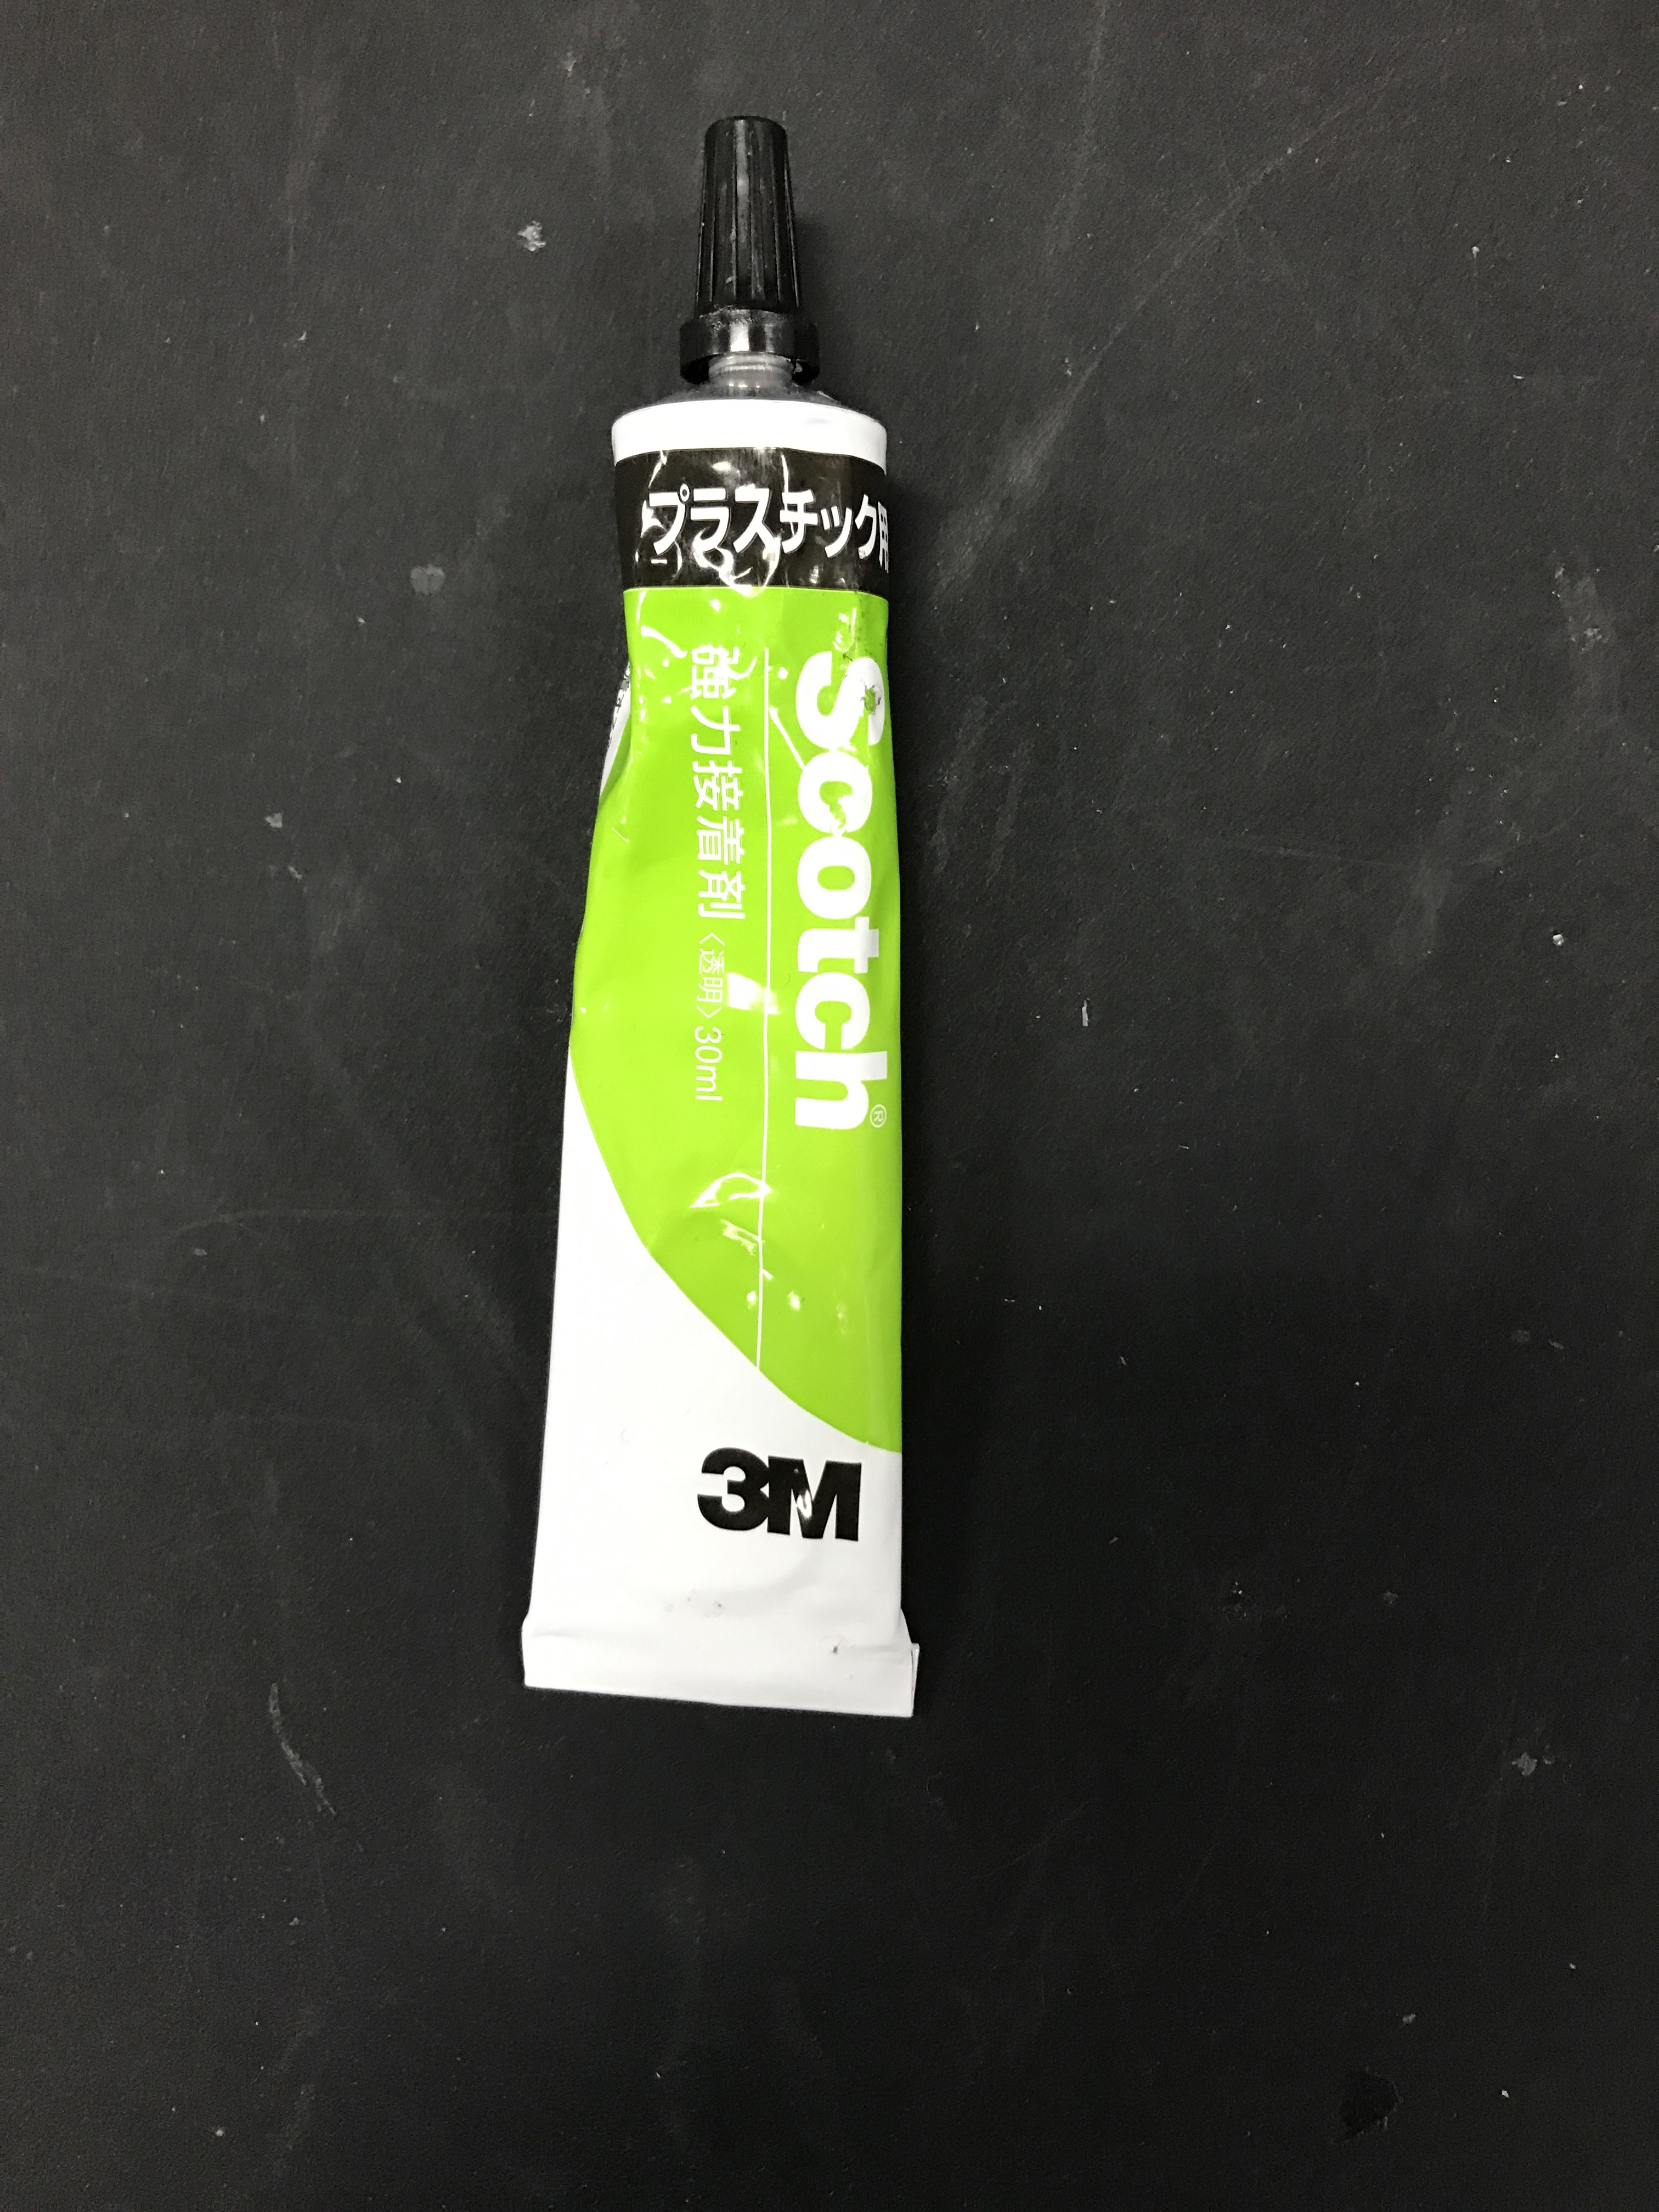
\includegraphics[width=140mm]{sc.JPG}
    \end{center}
  \caption{スコッチ強力接着剤}
 \label{fig:sc}
\end{figure}


\begin{figure}[htbp]
  \begin{center}
    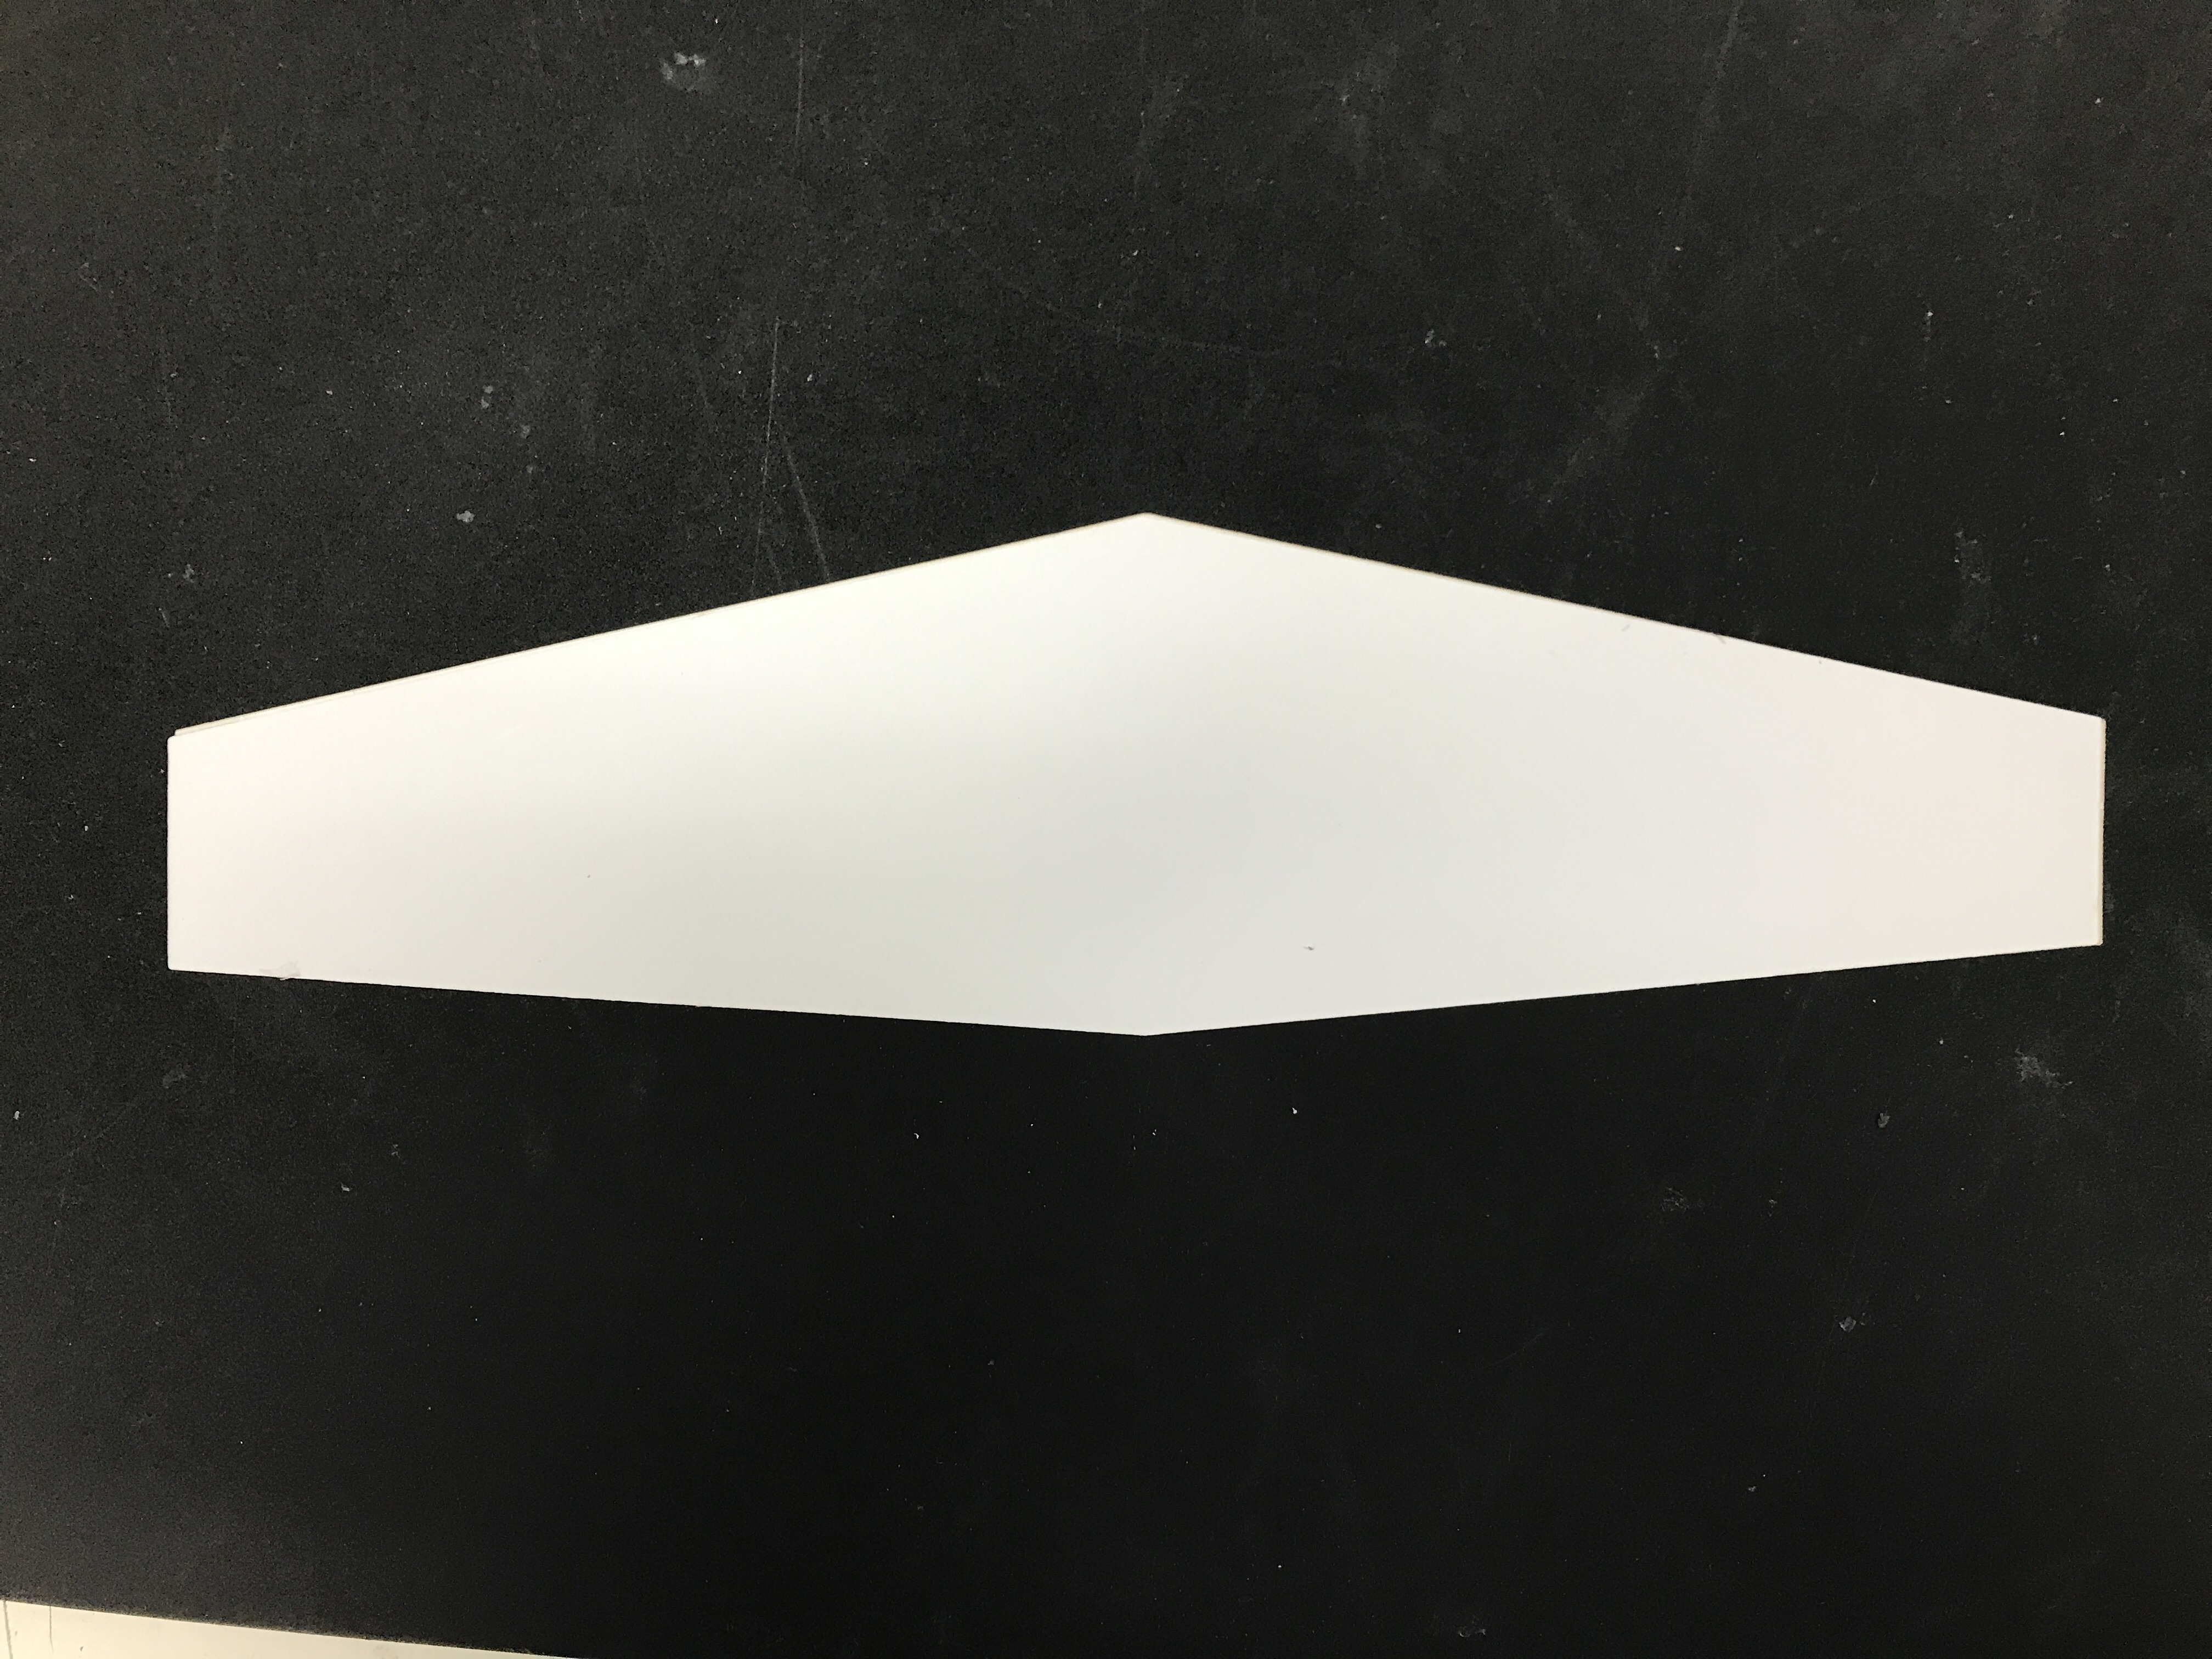
\includegraphics[width=140mm]{OK.JPG}
    \end{center}
  \caption{綺麗なつばさ}
 \label{fig:OK}
\end{figure}

\begin{figure}[htbp]
  \begin{center}
    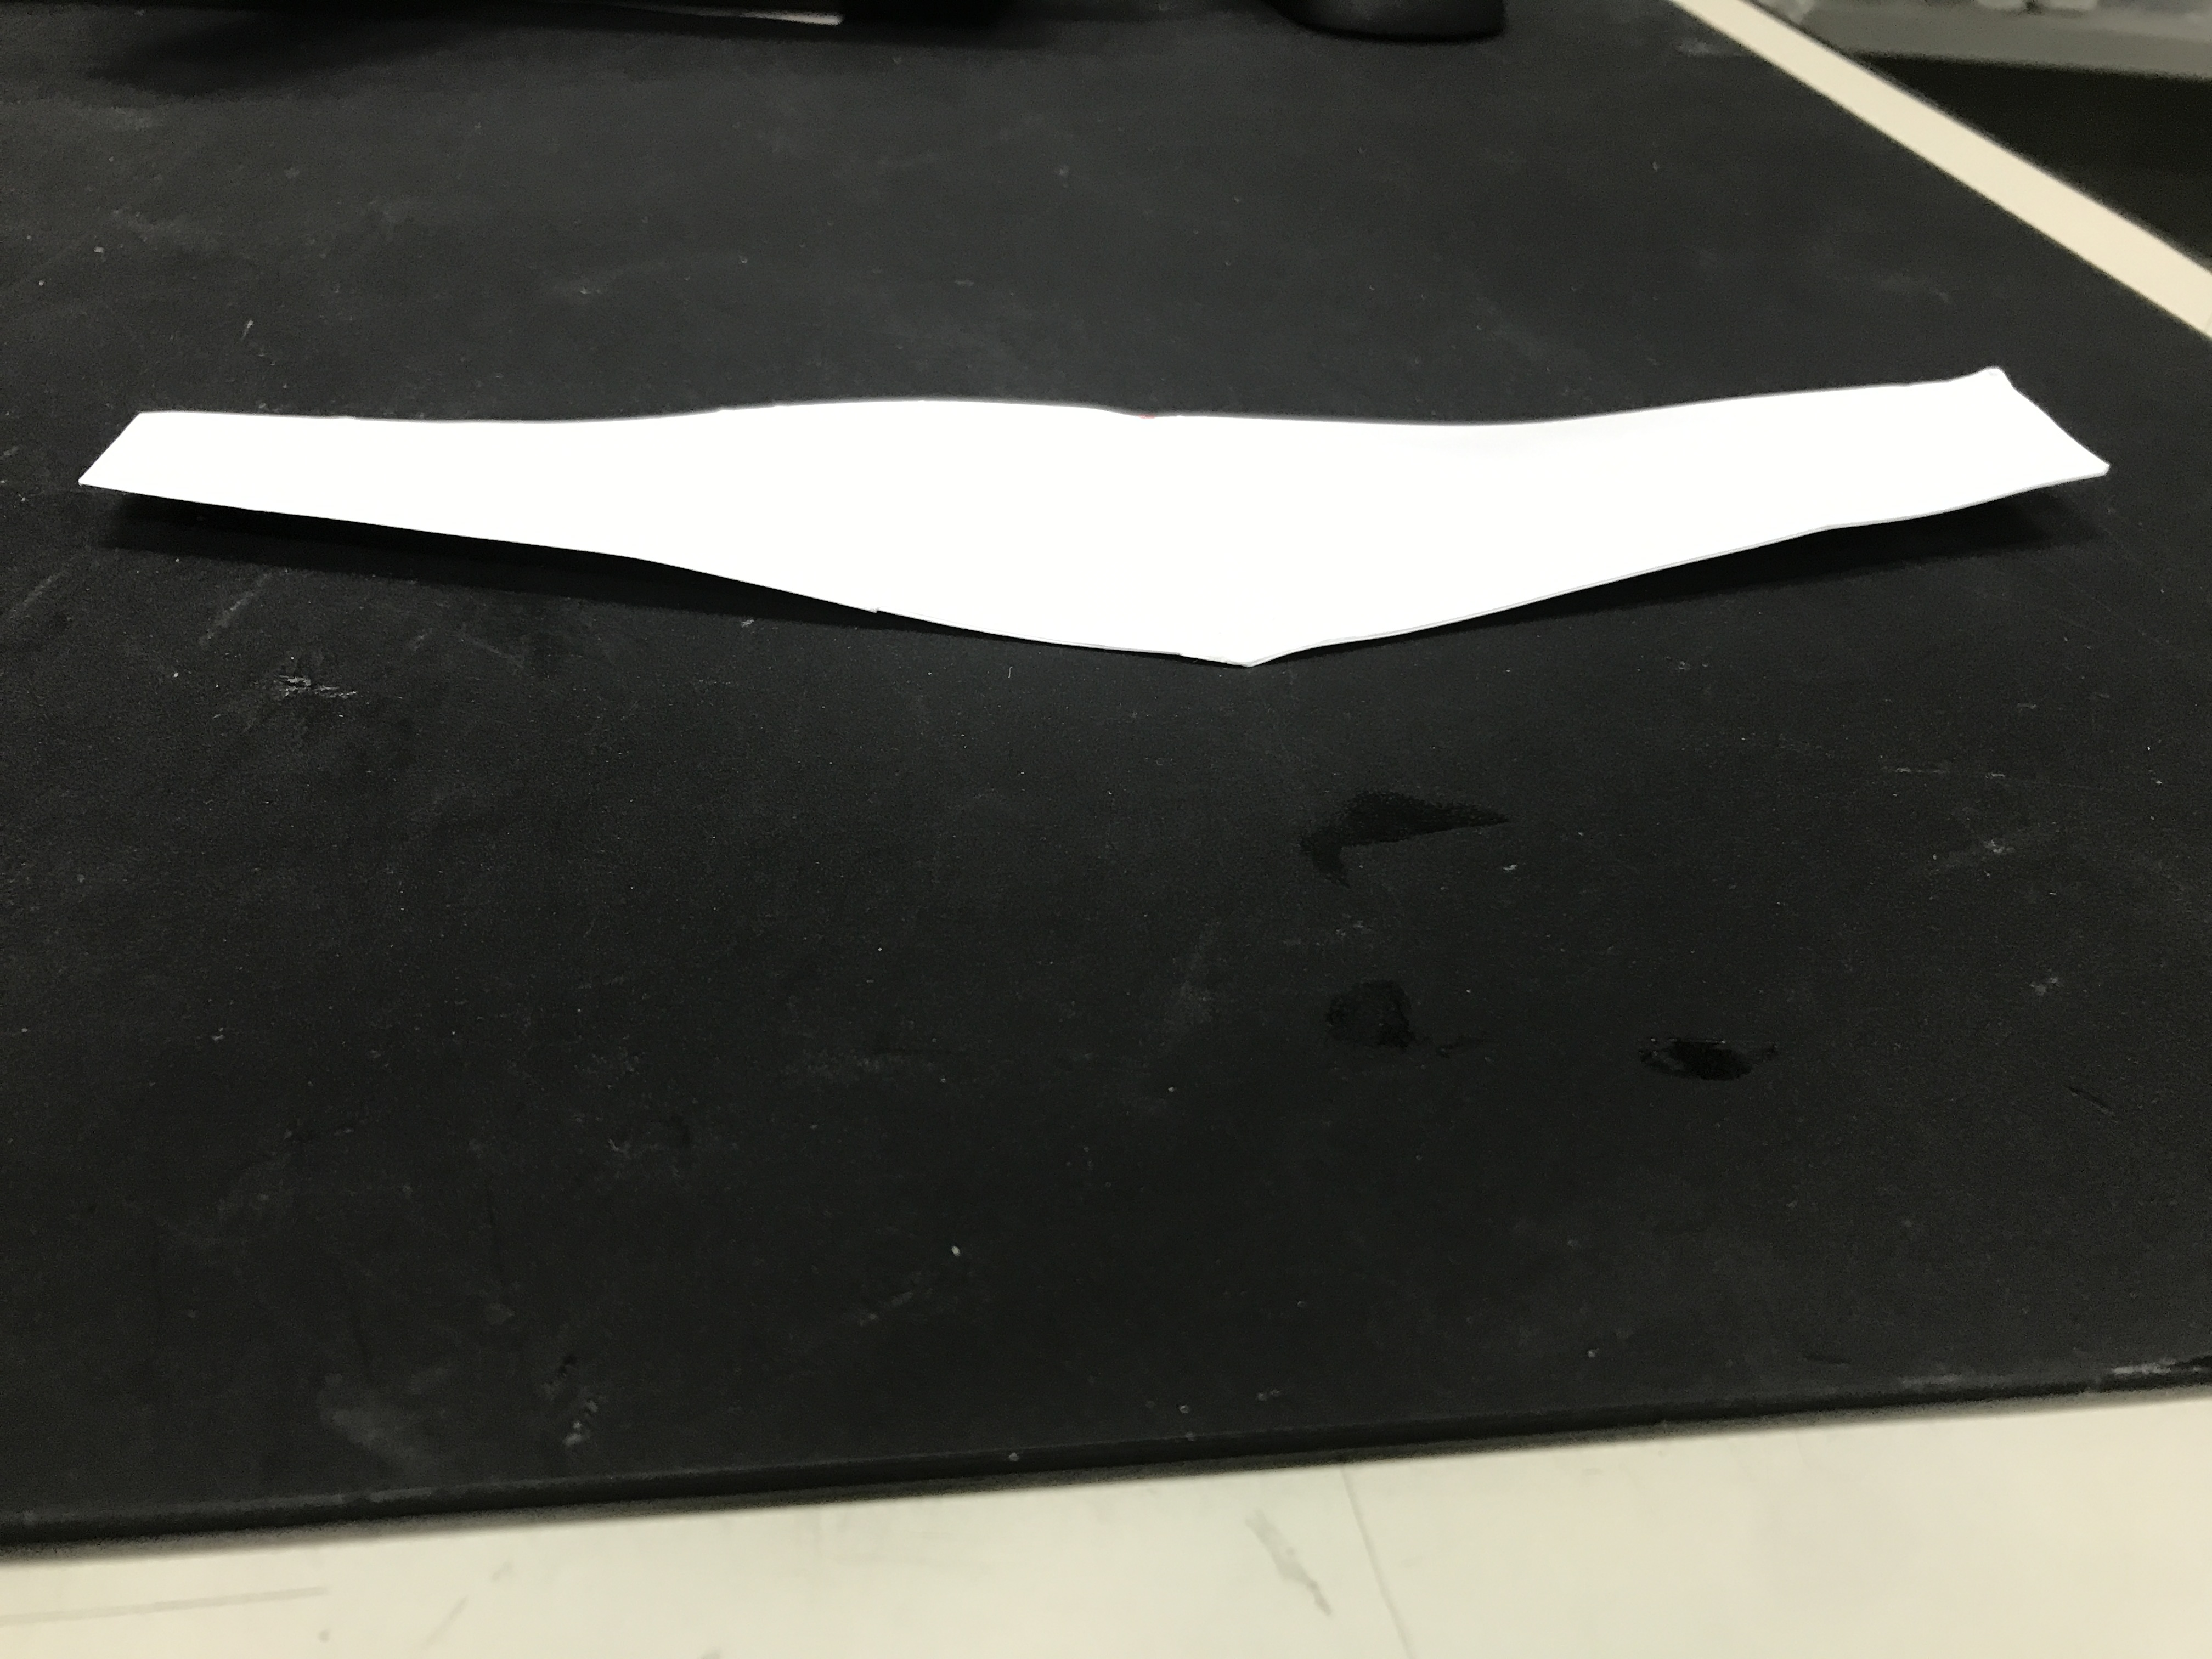
\includegraphics[width=140mm]{NG.JPG}
    \end{center}
  \caption{凸凹な翼}
 \label{fig:NG}
\end{figure}

\section{組み立て}
上記の方法で加工や接着を行った後組み立てを行う.翼をストローに張り付ける際,翼が傾かないようにしないといざ飛ばす時左に旋回したり右に旋回してしまうので注意が必要である.また水平に取り付けを行った場合でも左右に旋回する事がある.原因としては確認できない細かなズレのため生じている.そのため旋回したほうの主翼のエルロンを調整を行い旋回を修正していく必要がある.飛行機の各名称の図を図\ref{fig:er}に示す.
垂直尾翼に関しては尾翼と設置する面積が少ないため接着に安定感がなくすぐ折れてしまう.したがって図のようにテープを貼るなどして折れてしまわない工夫を行わないといけない.

\begin{figure}[htbp]
  \begin{center}
    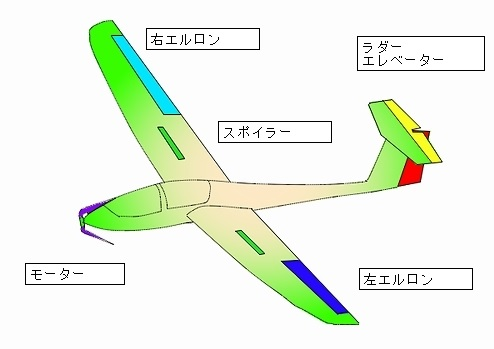
\includegraphics[width=140mm]{er.JPG}
    \end{center}
  \caption{飛行機の各名称}
 \label{fig:er}
\end{figure}

\chapter{飛行試験}

\section{実験の目的}
ストロー投射実験の目的はストロー単体と翼を付けた状態の飛行距離の変化を見るため行った.ストロー落下実験の目的はストローの抵抗を調べるため行った.飛行試験の実験目的は重心位置と空力中心の位置を変更した場合,飛行性能にどのような違いが発生するか調べるために

\section{実験の方法}
ストロー投射実験の実験方法はまず広い場所へ行きストローを投げる.投げた所から落ちた所までの距離を100回測り得られたデータをヒストグラムにまとめる.ストロー落下実験の実験方法は1500mmの高さからストローを落とし落下時間を計測する.この実験はストローを縦にした場合とストローを横にした場合それぞれ100回ずつ測定し得られたデータをヒストグラムにまとめる.飛行試験の実験方法はまず重心位置を変更するために先端に重量が違う重りを入れる事で重心位置を変更している.その後重心位置が重心位置より前の場合,重心位置が空力中心より後の場合,空力中心と重心位置が同じ場合の3種類の方法を試した.それぞれの方法で零戦とヘルキャットの飛行試験を100回行い得られたデータをヒストグラムにまとめる.

\section{実験結果}

\subsection{ストロー投射実験}
ストロー投下実験の結果,最大飛距離6920mm,最小飛距離2780mm,平均飛距離4150mmという結果になった.
下記にストロー投射実験から得た数値をもとに作成したヒストグラムを図(図\ref{fig:fly})に示す.

\begin{figure}[htbp]
  \begin{center}
    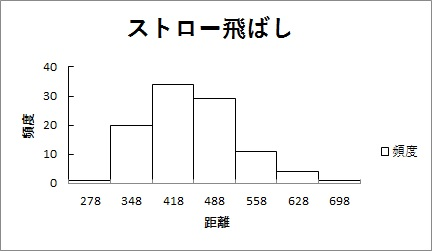
\includegraphics[width=90mm]{fly.JPG}
    \end{center}
  \caption{ストロー投射実験}
 \label{fig:fly}
\end{figure}

\subsection{ストロー落下実験横}
ストロー落下実験横の結果,最長時間0.89s,最短時間0.60s,平均時間0.75sという結果になった.
下記にストロー落下実験横から得た数値をもとに作成したヒストグラムを図(図\ref{fig:wide})に示す.

\begin{figure}[htbp]
  \begin{center}
    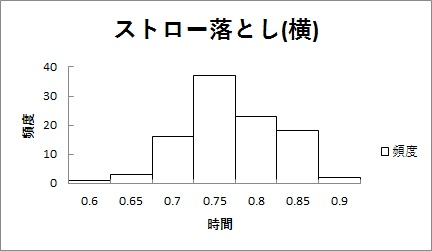
\includegraphics[width=90mm]{wide.JPG}
    \end{center}
  \caption{ストロー落下実験横}
 \label{fig:wide}
\end{figure}

\subsection{ストロー落下実験縦}
ストロー落下実験縦の結果,最長時間0.78s,最短時間0.47s,平均時間0.62sという結果になった.
下記にストロー落下実験縦から得た数値をもとに作成したヒストグラムを図(図\ref{fig:vertical})に示す.

\begin{figure}[htbp]
  \begin{center}
    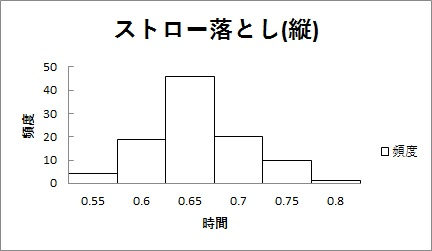
\includegraphics[width=90mm]{vertical.JPG}
    \end{center}
  \caption{ストロー落下実験縦}
 \label{fig:vertical}
\end{figure}

\subsection{重心位置が空力中心より前の場合}
\subsubsection{零戦}
重心位置が空力中心より10mm前の場合の零戦の飛行試験を行った結果,最大飛距離10060mm,最小飛距離4050mm,平均飛距離6101mmという結果になった.
下記に重心位置が空力中心より前の場合の零戦の飛行試験から得た数値をもとに作成したヒストグラムを図(図\ref{fig:zm})に示す.

\begin{figure}[htbp]
  \begin{center}
    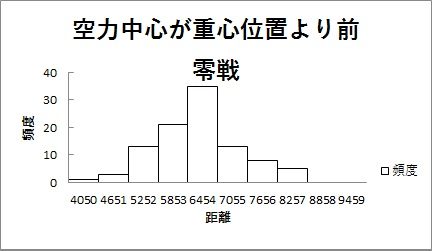
\includegraphics[width=90mm]{zm.JPG}
    \end{center}
  \caption{重心位置が空力中心より前の場合 零戦}
 \label{fig:zm}
\end{figure}

\subsubsection{ヘルキャット}
重心位置が空力中心より10mm前の場合のヘルキャットの飛行試験を行った結果,最大飛距離10040mm,最小飛距離4020mm,平均飛距離6090mmという結果になった.
下記に重心位置が空力中心より前の場合のヘルキャットの飛行試験から得た数値をもとに作成したヒストグラムを図(図\ref{fig:gm})に示す.

\begin{figure}[htbp]
  \begin{center}
    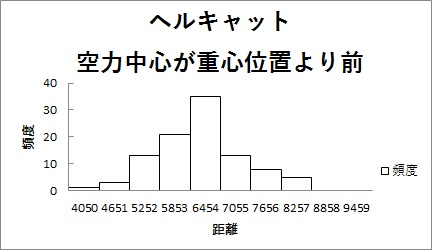
\includegraphics[width=90mm]{gm.JPG}
    \end{center}
  \caption{重心位置が空力中心より前の場合 ヘルキャット}
 \label{fig:gm}
\end{figure}

\subsection{重心位置が空力中心より後の場合}

\subsubsection{零戦}
重心位置が空力中心より7mm後の場合の零戦の飛行試験を行った結果,最大飛距離11040mm,最小飛距離4400mm,平均飛距離7250mmという結果になった.
下記に重心位置が空力中心より後の場合の零戦の飛行試験から得た数値をもとに作成したヒストグラムを図(図\ref{fig:zu})に示す.

\begin{figure}[htbp]
  \begin{center}
    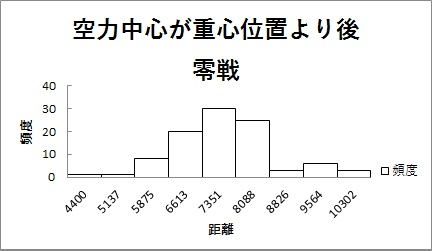
\includegraphics[width=90mm]{zu.JPG}
    \end{center}
  \caption{空力中心が重心位置より後の場合 零戦}
 \label{fig:zu}
\end{figure}

\subsubsection{ヘルキャット}
重心位置が空力中心より5mm後の場合のヘルキャットの飛行試験を行った結果,最大飛距離9510mm,最小飛距離4210mm,平均飛距離6650mmという結果になった.
下記に重心位置が空力中心より後の場合のヘルキャットの飛行試験から得た数値をもとに作成したヒストグラムを図(図\ref{fig:gu})に示す.

\begin{figure}[htbp]
  \begin{center}
    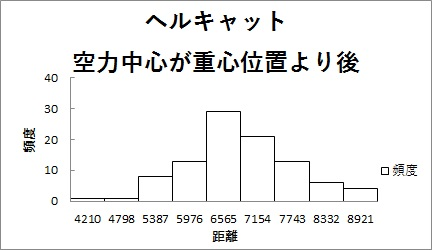
\includegraphics[width=90mm]{gu.JPG}
    \end{center}
  \caption{空力中心が重心位置より後の場合 ヘルキャット}
 \label{fig:gu}
\end{figure}

\subsection{重心位置と空力中心が同じ場合}

\subsubsection{零戦}
重心位置が重心位置が空力中心と同じ場合の零戦の飛行試験を行った結果,最大飛距離13210mm,最小飛距離4630mm,平均飛距離8100mmという結果になった.
下記に重心位置と空力中心が同じ場合の零戦の飛行試験から得た数値をもとに作成したヒストグラムを図(図\ref{fig:zo})に示す.

\begin{figure}[htbp]
  \begin{center}
    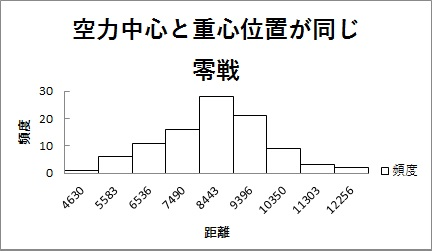
\includegraphics[width=90mm]{zo.JPG}
    \end{center}
  \caption{重心位置と空力中心が同じ場合 零戦}
 \label{fig:zo}
\end{figure}

\subsubsection{ヘルキャット}
重心位置が空力中心と同じ場合のヘルキャットの飛行試験を行った結果,最大飛距離9510mm,最小飛距離4210mm,平均飛距離6660mmという結果になった.
下記に重心位置と空力中心が同じ場合のヘルキャットの飛行試験から得た数値をもとに作成したヒストグラムを図(図\ref{fig:go})に示す.

\begin{figure}[htbp]
  \begin{center}
    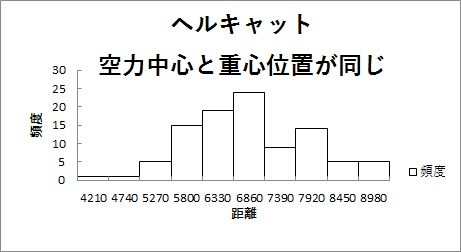
\includegraphics[width=90mm]{go.JPG}
    \end{center}
  \caption{重心位置と空力中心が同じ場合 ヘルキャット}
 \label{fig:go}
\end{figure}

\subsection{考察}
飛行試験を行った結果,ヘルキャットより零戦の方が航続距離が長いことが分かった.またストロー投射試験の平均飛距離より翼を付けた状態の機体の方が航続距離が長い.このことから翼から揚力が発生している事が分かる.
空力中心と重心位置の関係を調べた所,重心位置が空力中心より前にある場合は機体が頭上げの動作を行う,重心位置が空力中心より後にある場合は頭下げの動作を行う,重心位置と空力中心が同じ位置にある場合は頭上げ・下げの動作を行わないことが分かった.したがって重心位置と空力中心が同じ位置にある場合,理想の縦安定位置だと考える.

\chapter{おわりに}
目標だった長い距離とぶことが出来るストロー飛行機を作る事が出来たと考えている.具台的に零戦の最大飛距離は約13[m],ヘルキャットの最大飛距離は約10[m]という結果になった.実験結果からヘルキャットより零戦の方が航続距離が長い事が分かった.今回は時間がなく出来なかったが主翼の全長や翼弦の長さを変更した場合飛行距離にどのような影響が及ぶのか飛行試験してみたいところである.また,戦闘機以外にも旅客機など他の機体の種類も試してみたいと考えている.

\begin{thebibliography}{8}
\bibitem{sei} 牧野光雄,航空力学の基礎,産業図書株式会社,2016\slash{}07\slash{}15
\end{thebibliography}








\chapter*{謝辞}
\addcontentsline{toc}{chapter}{謝辞}
本論文作成にあたり研究の考え方,方法のまとめ方など長期にわたって熱意のあるご指導,ご鞭撻していただいた,伊藤恒平教授に厚く御礼申し上げます.

特に飛行機の原理や実験方法、また論文の書き方においても論文を何度も読んでいただき,指導していただいた伊藤恒平教授,に大変ご苦労をかけてしまいましたことにも心よりお詫び申し上げます.

その他,助けていただいた多くの皆様に心から感謝しております.ありがとうございました.




\end{document}






